%\documentclass[draftthesis,tocnosub,noragright,centerchapter,12pt]{uiucecethesis09}
\documentclass[tocnosub,noragright,centerchapter,12pt,fullpagesingle]{uiucecethesis09}
% Use draftthesis for notes and date markings on every page.  Useful when you
%   have multiple copies floating around.
% Use offcenter for the extra .5 inch on the left side. Needed with fullpage and fancy.
% Use mixcasechap for compatibility with hyperref package, which does NOT like all caps default
% Use edeposit for the adviser/committee on the title page.
% Use tocnosub to suppress subsection and lower entries in the TOC.
% PhD candidates use "proquest" for the proquest abstract.

\makeatletter

\usepackage{setspace}
\usepackage{epsfig}  % for figures
\usepackage{graphicx}  % another package that works for figures
\usepackage{subfigure}  % for subfigures
\usepackage{amsmath}  % for math spacing
%\usepackage{amssymb}  % for math spacing
%\usepackage{url}  % Hyphenation of URLs.
\usepackage{lscape}  % Useful for wide tables or figures.
\usepackage[justification=raggedright]{caption}	% makes captions ragged right - thanks to Bryce Lobdell

\usepackage{listings}

\lstset{language=[LaTeX]Tex,%C++,
    keywordstyle=\color{RoyalBlue},%\bfseries,
    basicstyle=\small\ttfamily,
    %identifierstyle=\color{NavyBlue},
    commentstyle=\color{Green}\ttfamily,
    stringstyle=\rmfamily,
    numbers=none,%left,%
    numberstyle=\scriptsize,%\tiny
    stepnumber=5,
    numbersep=8pt,
    showstringspaces=false,
    breaklines=true,
    frameround=ftff,
    frame=single
    %frame=L
}

% Uncomment the appropriate one of the following four lines:
\msthesis
%\phdthesis
%\otherdoctorate[abbrev]{Title of Degree}
%\othermasters[abbrev]{Title of Degree}

\title{TimeKeeper Documentation}
\author{Jereme Matthew Lamps}

% Advisor name is required for
% - doctoral students for the ProQuest abstract
% - master's students who do not have a master's committee
\advisor{Professor Matthew Caesar}

% Uncomment the \committee command for
% - all doctoral students
% - master's students who have a master's committee
%\committee{Professor Firstname Lastname, Chair\\
%        Professor Firstname Lastname} % etc.

\begin{document}

%%%%%%%%%%%%%%%%%%%%%%%%%%%%%%%%%%%%%%%%%%%%%%%%%%%%%%%%%%%%%%%%%%%%%%%%%%%%%%%
% COPYRIGHT
%
%\copyrightpage
%\blankpage

%%%%%%%%%%%%%%%%%%%%%%%%%%%%%%%%%%%%%%%%%%%%%%%%%%%%%%%%%%%%%%%%%%%%%%%%%%%%%%%
% TITLE
%
\maketitle

%\raggedright
\parindent 1em%

\frontmatter


%%%%%%%%%%%%%%%%%%%%%%%%%%%%%%%%%%%%%%%%%%%%%%%%%%%%%%%%%%%%%%%%%%%%%%%%%%%%%%%
% TABLE OF CONTENTS
%
\tableofcontents

\mainmatter

%%%%%%%%%%%%%%%%%%%%%%%%%%%%%%%%%%%%%%%%%%%%%%%%%%%%%%%%%%%%%%%%%%%%%%%%%%%%%%%
% INSERT REAL CONTENT HERE
%
\chapter{Introduction}
TimeKeeper is a small Linux Kernel patch, in conjunction with a Linux Kernel Module (LKM). TimeKeeper provides the ability to assign each container a $time\ dilation\ factor$, or TDF. A TDF of $n$ reduces the advancement rate of virtual time of the container by a factor of $n$. For example, if a container is assigned a TDF of 2, the container's virtual time will advance at half the rate of the wall-clock time. Conversely, if the container is assigned a TDF of .5, the container's virtual time will advance at twice the rate of the wall-clock time. This is done by modifying the $gettimeofday()$ system call, which is the most popular method of acquiring the current system time. TimeKeeper also provides a means of freezing (completely stopping execution) and unfreezing containers. When the containers are unfrozen, they will not perceive a change in time. In addition, TimeKeeper supports various functions to allow for integration with various network simulators. TimeKeeper provides the functionality to run $synchronized\ experiments$. A $synchronized\ experiment$ is defined as a collection of LXCs who may have varying TDFs, but their virtual times will be synchronized throughout the experiment.


If you plan to use either the CORE or ns-3 modifications, then reading Chapter 2 (Installation Guide) should be sufficient to use TimeKeeper. If you plan to develop or modify TimeKeeper, then the entire document should be read. 
	% for INTRODUCTION in "intro.tex"
\chapter{Installation Guide}
\label{chap:install}
After following the steps in the installation guide, TimeKeeper should be correctly installed on your system. This has been tested with Ubuntu 12.04 on both 32-bit and 64-bit systems. We are assuming you have the TimeKeeper source code.

\section{Setting up the Kernel}
\begin{itemize}
\item $cd\ /path/to/TimeKeeperSource$
\item $sudo\ ./kernel\_setup$ : This script will compile necessary scripts, download the linux-3.10.9 kernel (must have an internet connection to wget the linux kernel source) and store it in the /src directory. It will then make the necessary changes to the linux kernel.
\item Compile the newly modified kernel found at /src/linux-3.10.9. I have followed the instructions at: http://mitchtech.net/compile-linux-kernel-on-ubuntu-12-04-lts-detailed/.
\item When the modified kernel is compiled, restart the computer and load the modified kernel.
\end{itemize}

\section{Setting up CORE}
\begin{itemize}
\item $sudo\ ./core\_setup.sh$ : This script will install the necessary packages and compile CORE. You should not already have CORE installed on your system. 
\end{itemize}

\section{Setting up the TimeKeeper Kernel Module}
\begin{itemize}
\item $python\ setup\_module.py$ : The python script will ask you how many CPUs on your system you want to dedicate to TimeKeeper to use for an experiment. Then the TimeKeeper Kernel Module will be compiled. 
\end{itemize}
Congratulations! TimeKeeper is now installed.

\section{Simple Test}
With a simple test, we can see if TimeKeeper was correctly installed. 
\begin{itemize}
\item $sudo\ insmod\ ./TimeKeeper.ko$ : Insert the TimeKeeper Kernel Module into the Linux Kernel
\item $cd\ scripts$
\item $./print\_time <NumberOfLoops>$ : Run the print\_time script. This script simply does some computation, then prints out the PID, with how long it took to perform the computation in both virtual time and physical time (in format SECONDS:MICROSECONDS). This loop will be repeated NumberOfLoops. So run this for about 50 times. See figure \ref{fig:printtime} for sample print\_time output.
\item While print\_time is still running, open a new tab
\item $sudo\ ./timekeeper$-$dilate\ $-$r\ $-$p\ <pid>\ <TDF>$ : This script will dilate the process specified by PID, with a TDF specified by TDF. So use this command with the pid of the print\_time process, and a TDF of 2. 
\item Before the timekeeper-dilate command, the virtual time and physical time output of print\_time should be the same. When you dilate it, you will see the virtual time is now advancing at half the rate of physical time!
\item $sudo\ rmmod\ TimeKeeper$ : Remove the TimeKeeper Kernel Module
\end{itemize}
\begin{figure}[t]
      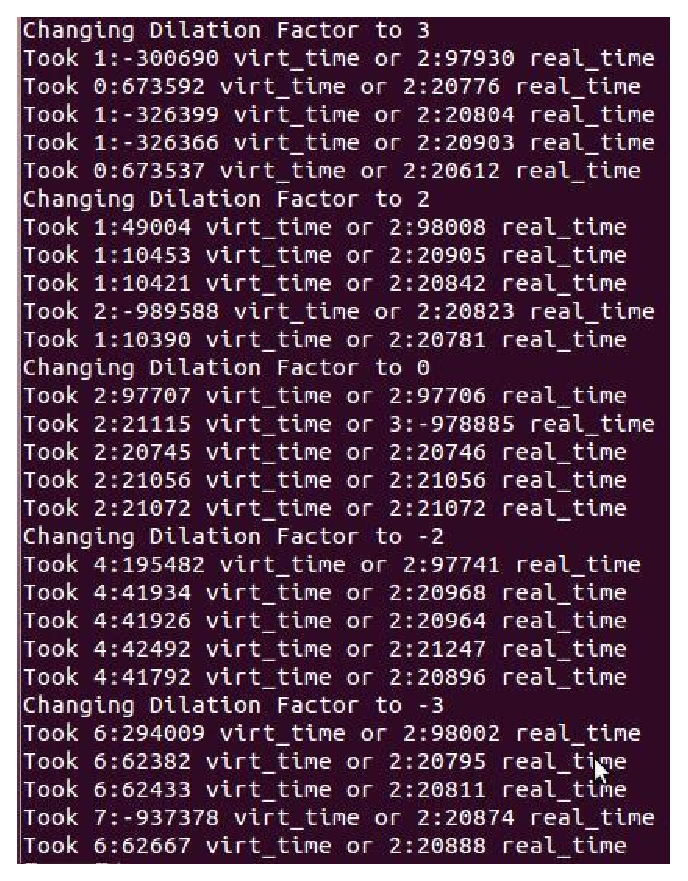
\includegraphics[width=\textwidth]{images/printtime.eps}
    \caption{Sample print\_time output }
    \label{fig:printtime}
  \end{figure}

\section{Simple CORE Experiment}
This section will explore starting a simple CORE experiment with TimeKeeper. 
\begin{itemize}
\item $sudo\ core$-$daemon\ $-$d$ : Start the CORE Daemon
\item $sudo\ insmod\ ./TimeKeeper.ko$ : Insert the TimeKeeper Kernel Module into the Linux Kernel
\item $sudo\ core$-$gui$ : Start the CORE gui. This needs to be ran as sudo to communicate with TimeKeeper
\item You should now see the CORE gui you are familiar with. You can add nodes to the GUI as you typically would. Double clicking on a host give you the ability to specify a TDF. This needs to be an integer value, see figure \ref{fig:coregui}.
\item When the topology is created, start the emulation by clicking the green 'play' button. This will create all containers, and assign them the TDFs you specified. Similar to the previous test, you may double click on a node in the gui, and run print\_time, verifying the difference between virtual time and physical time.
\item To start a synchronized experiment, navigate to the 'tools' tab, and select 'Synchronize Experiment'.
\item To stop the experiment, click on the red X
\item Remove the TimeKeeper Kernel Module when you exit out of the CORE GUI.
\end{itemize}
\begin{figure}[t]
      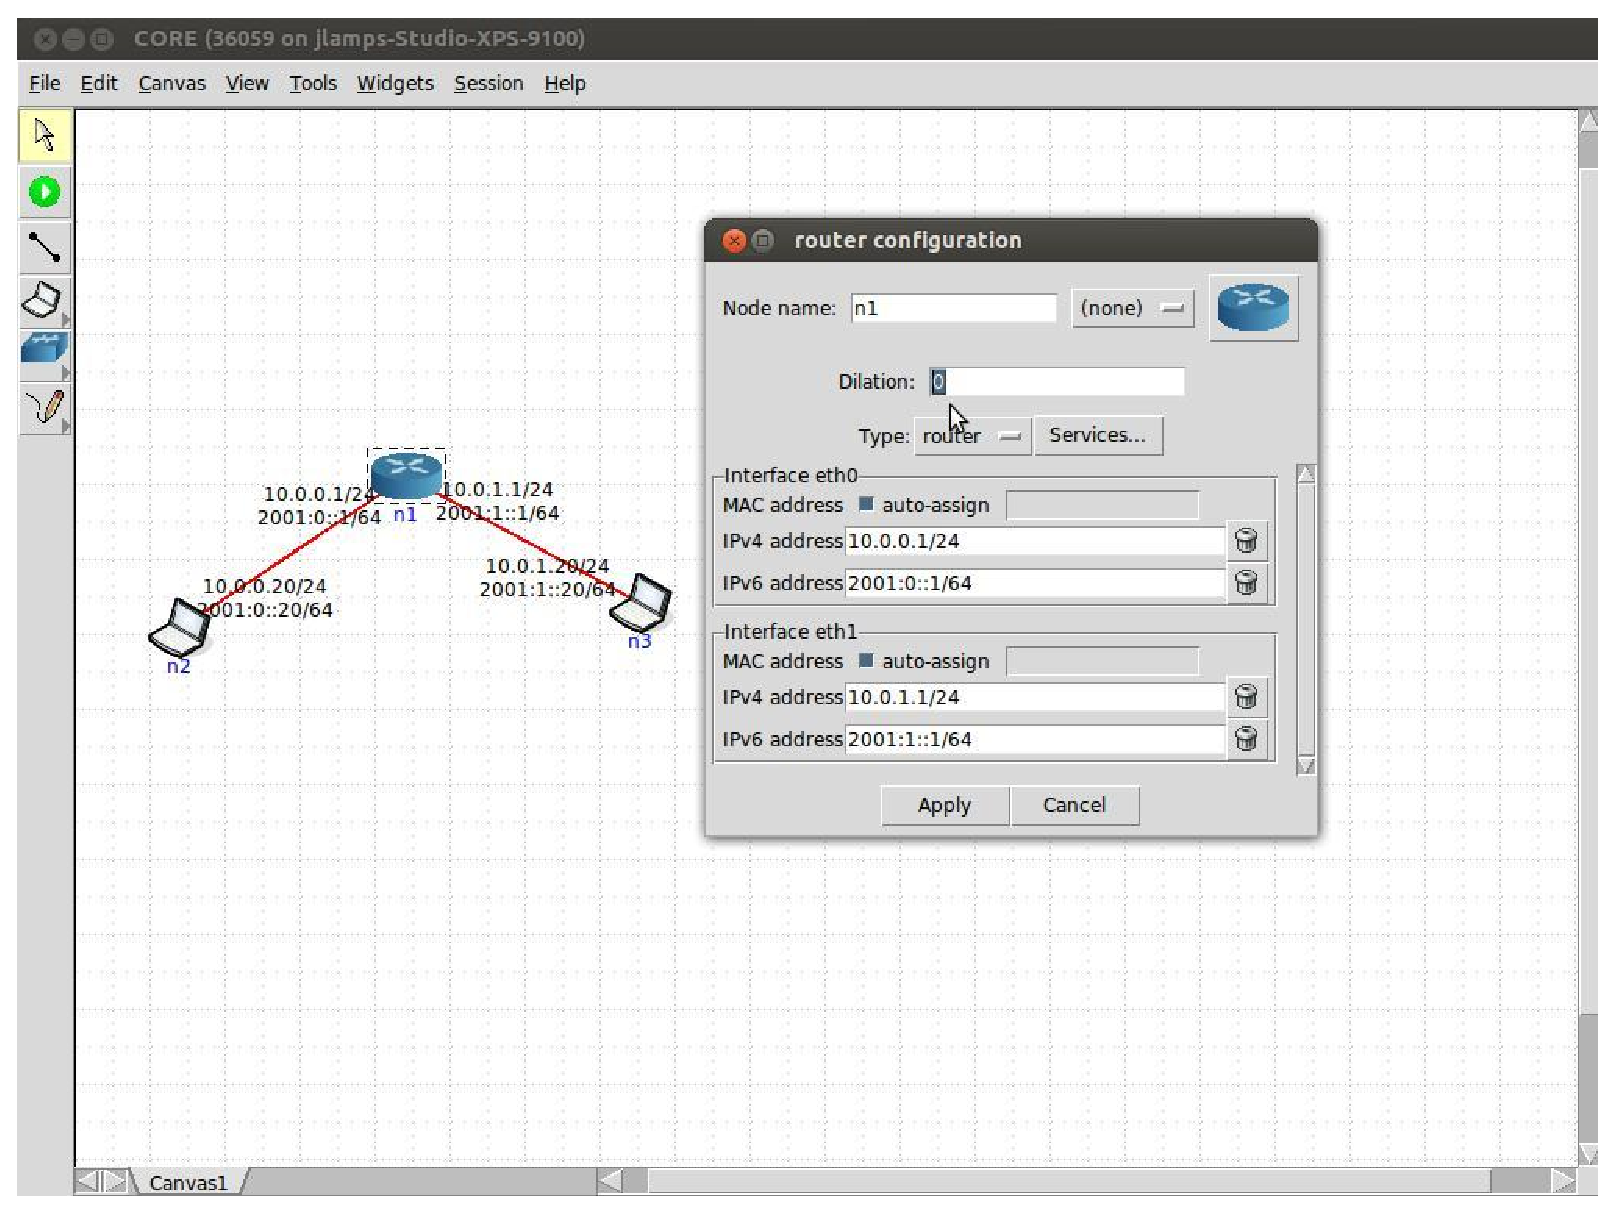
\includegraphics[width=\textwidth]{images/coregui.eps}
    \caption{CORE GUI with specifying a TDF}
    \label{fig:coregui}
  \end{figure}

\section{Simple NS-3 Experiment}
This section will describe how to start a simple ns-3 experiment with TimeKeeper with a CSMA network topology. This is assuming you already have ns-3 installed and set up on your system.
\begin{itemize}
\item $sudo\ apt$-$get\ install\ libreadline$-$dev$ : Install the necessary dependencies.
\item $cd\ /path/to/TimeKeeperSource/ns$-$3$
\item $make$ : Compile the scripts for easier LXC automation
\item $./lxcStarter\ <\#LXCs>\ <TDF>$ : When you run this command, \#LXCs will be created with the specified TDF and you will be given a prompt: 'Enter a command'.
\item Open a new terminal, and edit the file tap-csma-creator.py. Modify global variable PATH\_TO\_NS3\_TAP\_SRC and point it to the tapBridge source code within your ns-3's installation directory.
\item $python\ tap$-$csma$-$creator.py\ <\#LXCs>\ <simulatorTDF>$ : This script will create a .cc file for ns-3, with the correct number of LXCs, as well as specifying the TDF of the simulator. 
\item Move to where your ns-3 installation is, and run: $./waf\ --run\ tap$-$csma$-$virtual$-$machine$ then wait for the words TimeKeeper Integration Complete.
\item Return to the terminal where lxcStarter is running, and type $start$, this will tell TimeKeeper to start the synchronized experiment.
\item From lxcStarter, you can now send specific commands to each lxc, or all of them at once. For example, lets say you passed in the value 2 when you started lxcStarter. This will create 2 LXCs, named lxc-1 and lxc-2 with ip addresses 10.0.0.1 and 10.0.0.2 respectively. To view currently running processes within lxc-1, you would type '1 ps -A'. The first number means to send the command to lxc-1, everything after that will be what gets executed on the specified LXC. The output will be directed to /tmp/lxc-1.output. Likewise, if you want to see the files in the current directory of lxc-2, you then run '2 ls -l', and the output of the command will get written to /tmp/lxc-2.output. You can also send the same command to all LXCs at once (if you have thousands running for example) simply do '$all\ <command>$' ie: 'all ifconfig' will perform ifconfig on every LXC, and output it to /tmp/lxc-\#.output.  
\item When you are done with the experiment, send $exit$ to the lxcStarter process.
\end{itemize}


\chapter{User API}
\label{chap:design}
TimeKeeper comes with a simple and intuitive set of functions to create and manage time-dilated containers. The presented API describe the set of functions TimeKeeper provides to the user. The functions are defined in scripts/TimeKeeper\_functions.h. You can ignore this section if you are going to use TimeKeeper with the CORE or ns-3 modifications, as everything is handled internally.

\section{General Functions}
\begin{description}
 \item[clone\_time(unsigned long flags, float dilation, int should start) ] \hfill \\
 The $clone\_time()$ function will cause a new process to be cloned from the calling process. The $flags$ argument is a bitmap of various tunable knobs similar to the $clone()$ system call. The $dilation$ argument represents the dilation factor of this new process. The $should\_start$ argument determines if the new time-dilated process should be allowed to start running immediately or not. A $should\_start$ value of 0 means the process will immediately start, while a $should\_start$ value of 1 means the new process should not immediately start. Not immediately starting a new process may be useful if you wish to clone numerous time-dilated processes, but need them all to start running at the same point in physical time (as you may need to do in an $experiment$).
 \item[dilate(int pid, float dilation) ] \hfill \\
 The $dilate()$ function will change the TDF of a process. The $pid$ argument represents the unique process identifier of the process whose TDF you wish to change. The $dilation$ argument represents the new dilation factor of the process. This function can be called on both a process that was instantiated through the $clone\_time()$ function, as well as any standard Linux process.
 \item[dilate\_all(int pid, float dilation) ] \hfill \\
The $dilate\_all()$ function will do the same thing as the $dilate()$ function, but in addition will recursively set the TDF of every child and grandchild of the process. 
 \item[freeze(int pid)] \hfill \\
The $freeze()$ function will stop a process from continuing to execute on the processor. The current system time in which it was frozen is stored in the process's corresponding $task\_struct$.
\item[freeze\_all(int pid) ] \hfill \\
The $freeze\_all()$ function will do the same thing as the $freeze()$ function, but in addition will recursively freeze every child and grandchild of the process. 
 \item[unfreeze(int pid) ] \hfill \\
The $unfreeze()$ function allows a previously frozen process to be unfrozen and continue execution. In between the time in which the process was frozen and unfrozen, the process will not perceive any passage of time. For example, if a process was frozen at time 30 seconds, and unfrozen at time 40 seconds, it will resume its execution at time 30 seconds. 
\item[unfreeze\_all(int pid) ] \hfill \\
The $unfreeze\_all()$ function will do the same thing as the $unfreeze()$ function, but in addition will recursively unfreeze every child and grandchild of the process. 
\item[leap(int pid, int otherPid) ] \hfill \\
The $leap()$ function changes the process's virtual time specified by $pid$ to be identical to that of the process with the given id $otherPid$. When this is applied to a process that is currently frozen, the process will essentially leap over an epoch of virtual time, without needing to directly modify its TDF. 
\item[gettimepid(int pid, struct timeval tv, struct timezone tz) ] \hfill \\
The $gettimepid()$ function will query the current virtual time of the process specified by the $pid$. This can be queried on a process with a TDF or without a TDF.
\item[gettimename(char *lxcname, struct timeval tv, struct timezone tz) ] \hfill \\
The $gettimename()$ function is the same as the $gettimepid()$ function, but it takes an LXC name instead of a $pid$. 
\item[gettimeofdayoriginal(struct timeval tv, struct timezone tz) ] \hfill \\
The $gettimeofdayoriginal()$ function will return the actual system time, regardless of whether the calling process is time-dilated or not. This is useful mainly for debugging, when you want to verify the virtual time is being scaled appropriately with respect to the system time.
\end{description}
\begin{figure}[t] 
      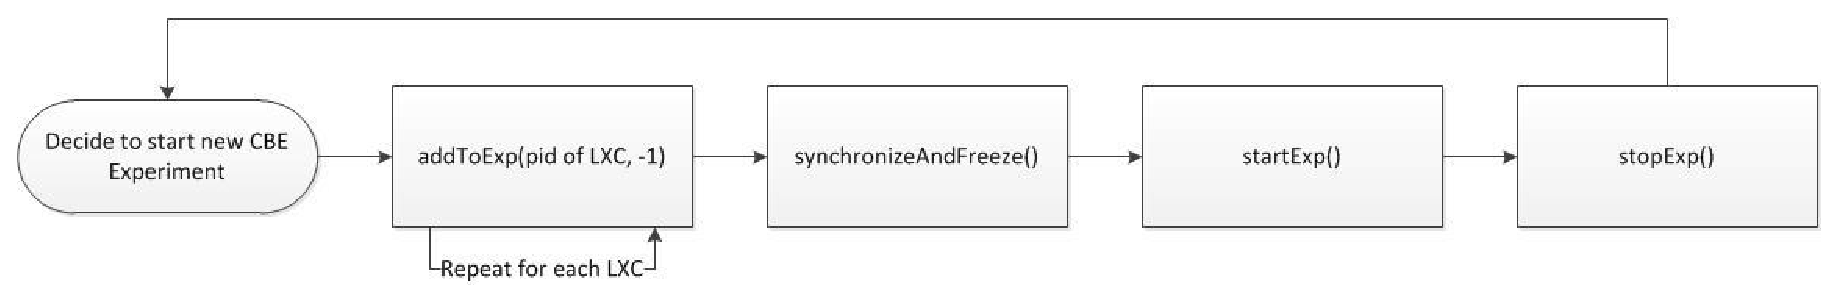
\includegraphics[width=\textwidth]{images/cbe_functions.eps} 
    \caption{Order of Operations to Setup a CBE Experiment } 
    \label{fig:cbe_functions} 
  \end{figure} 
\begin{figure}[t] 
      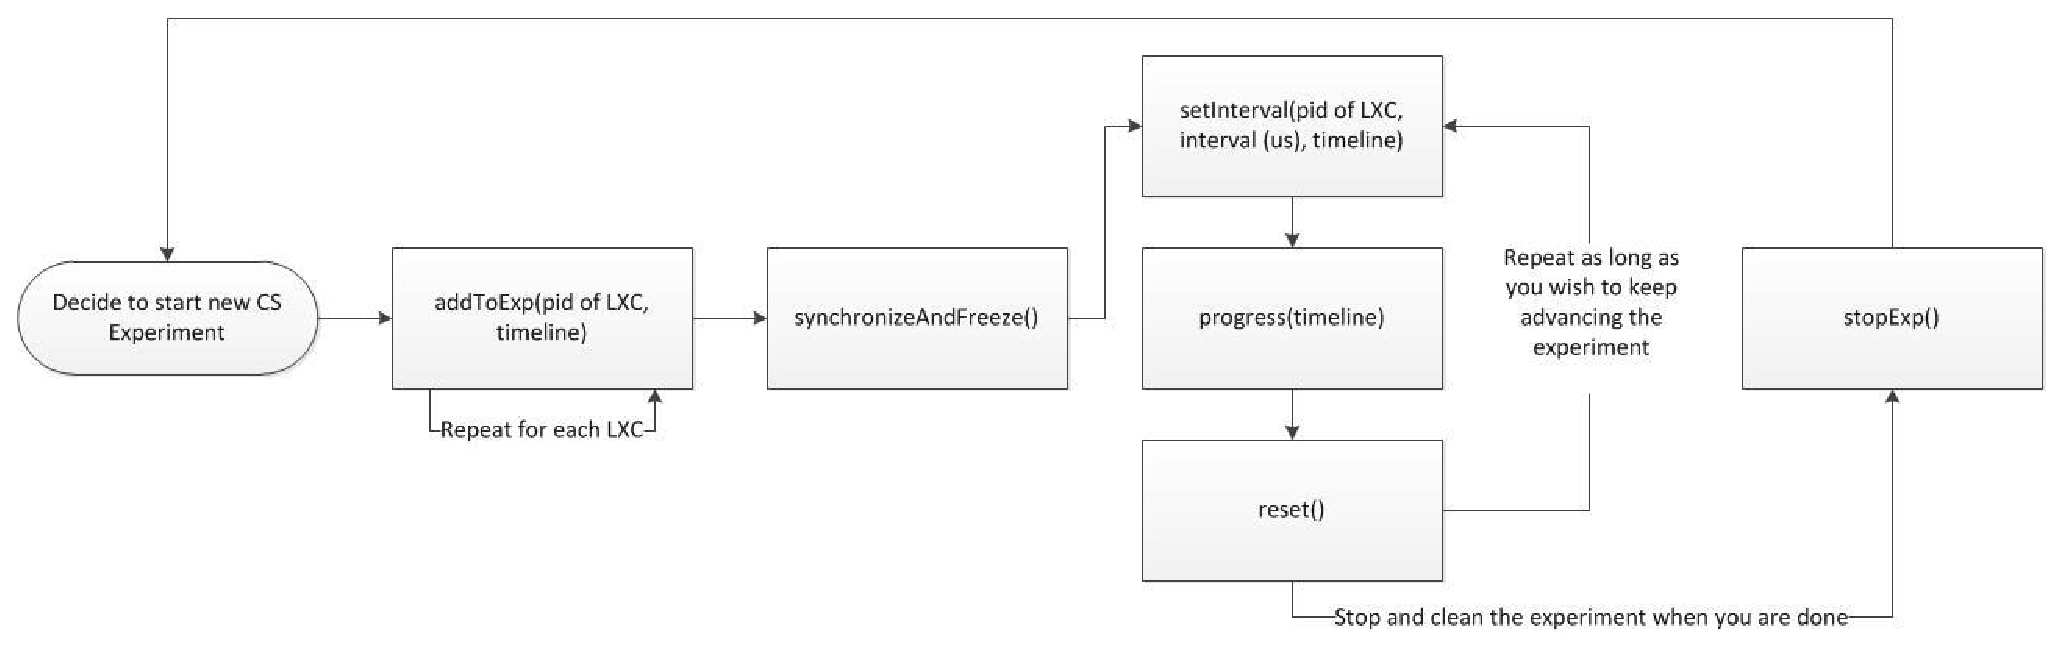
\includegraphics[width=\textwidth]{images/cs_functions.eps} 
    \caption{Order of Operations to Setup a CS Experiment } 
    \label{fig:cs_functions} 
  \end{figure} 
\section{Experiment Synchronization Methods}
TimeKeeper supports two methods to perform experiment synchronization. They are discussed below.
\subsection{Concurrent Best Effort}
Concurrent Best Effort (CBE) is when the emulated nodes and the network simulator run side by side. The network simulator is tied to some external clock (usually the system clock), and advances at the same rate as the emulated nodes. The simulator will make a best effort to deliver packets when it should. If a packet is too late, the simulator may send the packet as soon as it can, or simply drop the packet. In a CBE experiment, the simulator is not aware of TimeKeeper, and does not need to directly interact with it. Any experiments conducted with the CORE or ns-3 simulator utilizes the CBE method.
\subsection{Concurrent Synchronization}
With Concurrent Synchronization (CS) the simulator directly communicates with TimeKeeper, and specifies how far each LXC's virtual time should be allowed to advance in the following round. When the round is started, the simulator executes all events within that interval (the current virtual time and the virtual time to which each LXC will advance to). At the end of each round, the simulator may respecify how far each LXC can progress in virtual time, then start a new round. The CS method was utilized when TimeKeeper was integrated with S3F.

\section{Experiment Synchronization Functions}
The following functions were developed to support both CBE and CS experiments. The order of operations to perform a CBE experiment is outlined in Figure \ref{fig:cbe_functions}, while the order of operations to perform a CS experiment is outlined in Figure \ref{fig:cs_functions}. You should be careful and try not to mix functions (trying to call both $startExp()$ and $setInterval()$ in the same experiment), as this may give inaccurate results.
\begin{description}
\item[addToExp(int pid, int timeline) ] \hfill \\
The $addToExp()$ function call will add the given $pid$ of the LXC to the experiment. If a $timeline$ is supplied, it means you are going to try to start a CS experiment. If $timeline$ is less than 0, you will be setting up a CBE experiment. 
\item[synchronizeAndFreeze() ] \hfill \\
Once all of the LXCs have been added to the experiment, the $synchronizeAndFreeze()$ function is called, which will freeze all of the LXCs, and set all of their virtual times to be at the same starting point. 
\item[startExp()] \hfill \\
The $startExp()$ function will start a synchronized experiment with TimeKeeper. The prerequisite functions of $addToExp()$ and $synchronizeAndFreeze()$ are necessary before calling this function.
\item[setInterval(int pid, int interval, int timeline) ] \hfill \\
The $setInterval()$ function will specify the interval in which you wish an LXC will advance in virtual time. The $pid$ represents the $pid$ of the LXC, $interval$ represents the virtual time advancement in microseconds, and the $timeline$ value must correspond to the timeline associated with the LXC. 
\item[progress(int timeline, int force) ] \hfill \\
The $progress()$ function will progress all LXC's virtual times by the amount specified by the $setInterval()$ function and associated with the given $timeline$. If an LXC has not been assigned an interval with the $setInterval()$ function, then its virtual time will not progress. The function will return when all LXCs associated with the given $timeline$ had advanced to the correct virtual time. If $force$ is 0, then TimeKeeper will do a best effort to bring each LXC to the correct virtual time. However, there may be a certain amount of error, as the underlying mechanism for freezing and unfreezing is not 100\% accurate. If $force$ is 1, each LXC's virtual time will progress to precisely the exact moment in virtual time in which it should. This is done by changing each LXC's virtual time after it is frozen.
\item[reset(int timeline) ] \hfill \\
The $reset()$ function will reset all previously set intervals for all LXCs on the given $timeline$. 
\item[stopExp()] \hfill \\
The $stopExp()$ function call will stop a running experiment. This will be used after the experiment has finished, and you wish to clean up TimeKeeper. Once TimeKeeper is cleansed with this function, you may proceed to set up a new experiment.
\end{description}

\section{Utility Scripts}
In addition to the API, simple utility scripts were created to perform TimeKeeper commands from the command line. They are located in /path/to/TimeKeeper/scripts.
\begin{description}
 \item \textbf{timekeeper-dilate [-r] [-p pid] [-n name] TDF} \hfill \\
	Sets the TDF of a process. -r dilates all children of the process as well. You may use either -p to specify a pid, or -n to specify the LXC name. 
 \item \textbf{timekeeper-freeze [-r] pid} \hfill \\
	Freezes a process specifed by pid. -r will freeze all children of the process as well.
 \item \textbf{timekeeper-unfreeze [-r] pid} \hfill \\
	Unfreezes a process specifed by pid. -r will unfreeze all children of the process as well.
 \item \textbf{timekeeper-gettime [-p pid] [-n name]} \hfill \\
	Returns the current time of a process. You may use either -p to specify a pid, or -n to specify the LXC name. 

 \item \textbf{timekeeper-addToExperiment [-t timeline] [-d tdf] [-p pid] [-n name]} \hfill \\
	Adds a process to an experiment. You may use -t to specify a timeline, and -d to specify a TDF. You may use either -p to specify a pid, or -n to specify the LXC name.
 \item \textbf{timekeeper-synchronizeAndFreeze} \hfill \\
	Will freeze all of the processes added to the experiment, and set their virtual times to be the same
 \item \textbf{timekeeper-startExperiment} \hfill \\
	Starts a CBE experiment.
 \item \textbf{timekeeper-setInterval [-p pid] [-n name] TIMEus timeline} \hfill \\
	Sets the virtual time progression of a process. You may use either -p to specify a pid, or -n to specify the LXC name. The TIME is in microseconds. 
 \item \textbf{timekeeper-progress [-f] [-t timeline]} \hfill \\
	Progresses all LXCs associated with the specified timeline. -f flag will force the process to advance at the exact interval. 
 \item \textbf{timekeeper-reset [-t timeline]} \hfill \\
        Resets all progression interviews associated with a timeline
 \item \textbf{timekeeper-stopExperiment} \hfill \\
	Stops an experiment
\end{description}

\chapter{Technical Details} 
\label{chap:implementation}

This section delves into TimeKeeper's implementation. This section should be read if you plan to modify the TimeKeeper source code. TimeKeeper's implementation can broken up into distinct components: the Linux Kernel modifications, the TLKM, and the integration of TimeKeeper with various network simulators. This chapter will describe each of these components in detail.
\begin{figure}[t] 
      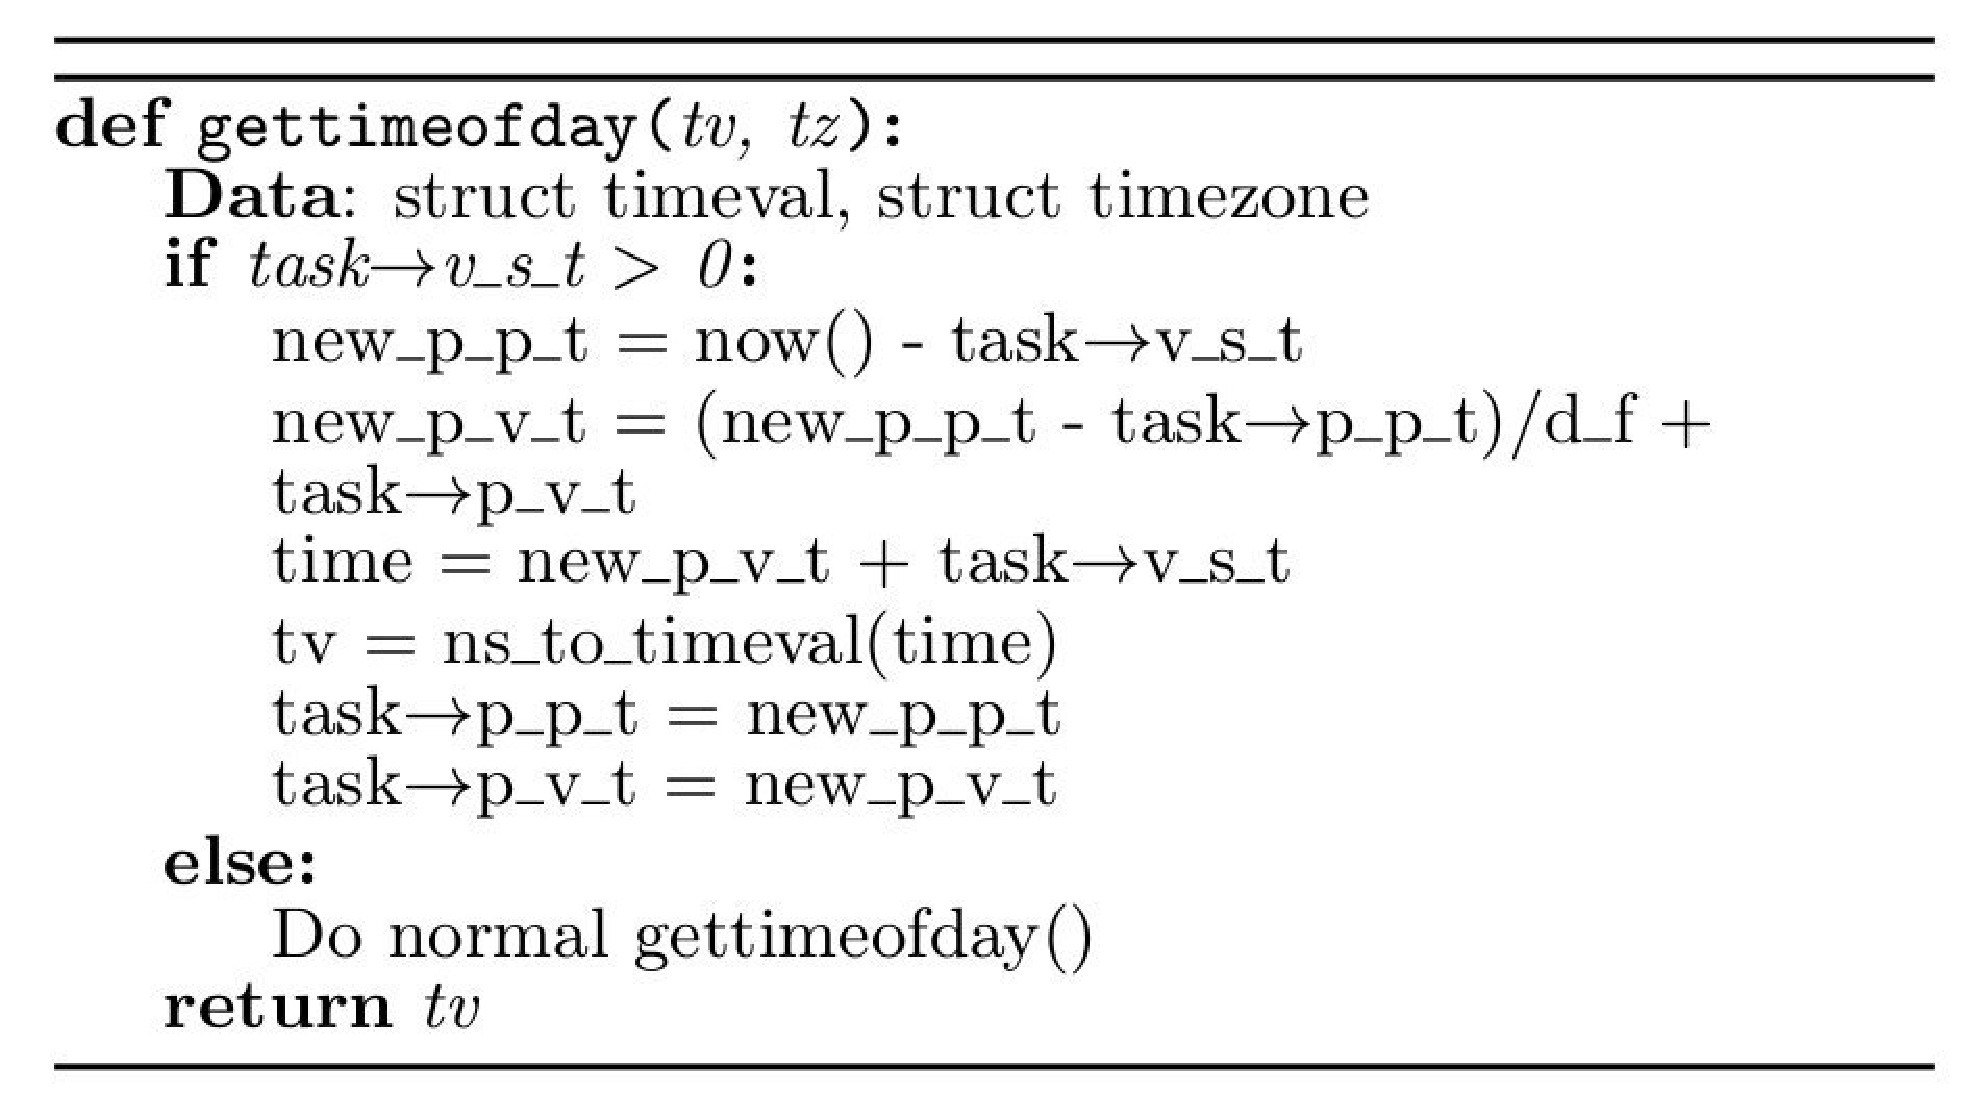
\includegraphics[width=\textwidth]{images/gettimeofday_alg.eps} 
    \caption{Pseudocode For Modified Getttimeofday System Call} 
    \label{fig:gettimeofday_alg} 
  \end{figure} 
\begin{figure}[t] 
      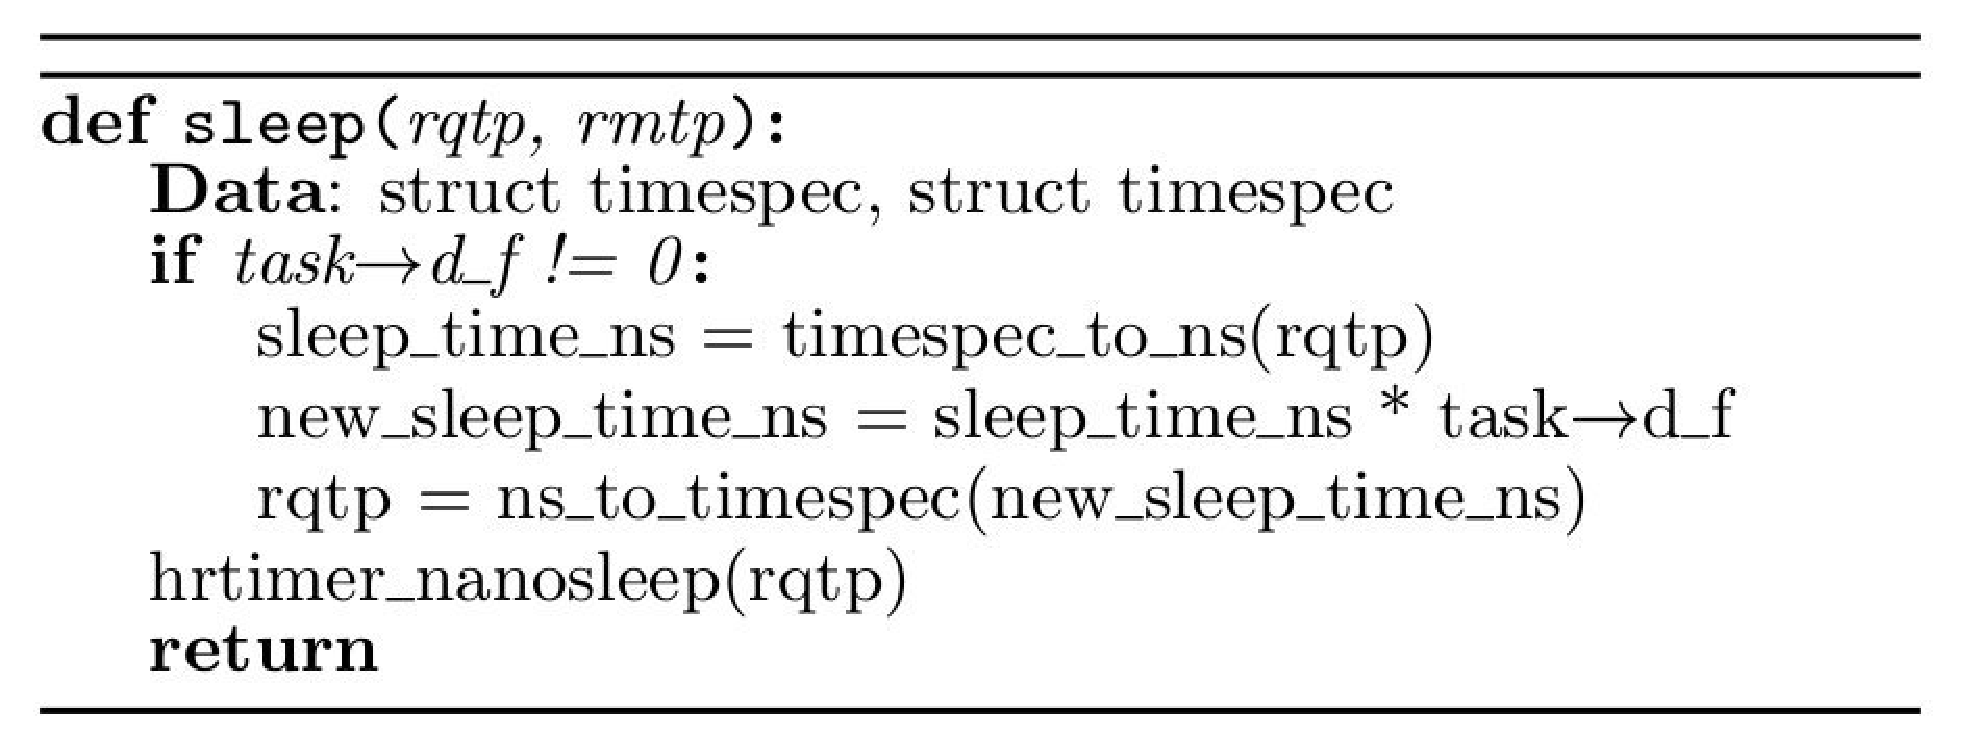
\includegraphics[width=\textwidth]{images/sleep_alg.eps} 
    \caption{Pseudocode For Modified Nanosleep System Call} 
    \label{fig:sleep_alg} 
  \end{figure} 
\section{Kernel Modifications}
\label{sec:kernel_modifications}
In this section, we will discuss the purpose of each modified file in the Linux Kernel, the reason why we needed to modify that particular file, as well as describe the changes made. All of our kernel modifications were made to a 32-bit 3.10.9 Linux Kernel, then extended to work on a 64-bit Linux Kernel as well.
\subsection{32-bit TimeKeeper}
\begin{description} 
\item[linux-3.10.9/include/linux/init\_task.h] \hfill \\
        The $init\_task.h$ file defines many structures having to do with an individual process. Most importantly for us, it initializes all variables in the Linux $task\_struct$ structure. There exists a $task\_struct$ for every running process in Linux, and it maintains important information pertaining to that particular process. It was within this structure where we added six additional variables (44 bytes) in order for each process to maintain its own notion of virtual time. The variables added are:
        \begin{itemize} 
                        \item 4 bytes $dilation\_factor (d\_f)$ represents the TDF of the process. It may be either positive or negative. It is important to realize a TDF is represented as an $integer$ within the Linux Kernel, but as a $float$ from a user's perspective. This is because doing floating point calculations from within the Linux Kernel is very difficult, and it is recommended not be be done. Therefore, when a user supplies a TDF as a float, it will be converted to an integer before it is used in virtual time calculations. This process is completely transparent from the user's perspective.
                \item 8 bytes $virtual\_start\_time (v\_s\_t)$ represents the point in system time (in ns) in which the process started progressing in virtual time by a scaled factor of its TDF.
                \item 8 bytes $past\_virtual\_time (p\_v\_t)$ represents how far virtual time has progressed from the $v\_s\_t$ since the last time the process inquired about the current time.
                \item 8 bytes $past\_physical\_time (p\_p\_t)$ represents how far physical time has progressed from the $v\_s\_t$ since the last time the process inquired about the current time.
                \item 8 bytes $freeze\_time (f\_t)$ is used to determine if the process is currently frozen or not. If the value of $freeze\_time$ is zero, then the process is currently not frozen. If the process is currently frozen, then $freeze\_time$ will be set to the point in time (in ns) in which the process was frozen. This variable is kept entirely internal to TimeKeeper. 
	\item 8 bytes $wakeup_time (w\_t)$ variable is used to ensure the process sleeps for the appropriate amount of time, regardless of whether or not it is in an $experiment$ or not. The need for this variable is further discussed in Section \ref{sec:hooking}.
        \end{itemize}
        How these variables interact with each other to give the process a different perception of time will be explained in later sections. 
\item[linux-3.10.9/linux/kernel/time.c] \hfill 
        \begin{itemize} 
                        \item \textbf{gettimeofday()} \\
                        The $gettimeofday()$ system call allows a user-land process to determine the current system time to within microsecond accuracy. The $gettimeofday()$ system call is one of the only ways for a process to determine the current system time, and it is the most popular method. Therefore, in order to change a process's perception of time, we modify this system call to return a different time from the system time, which is based on the calling process's TDF. See Figure \ref{fig:gettimeofday_alg} for the algorithm. If the process who calls $gettimeofday()$ has its $virtual\_start\_time$ set, then the modified virtual time will be returned. If the process does not have the $virtual\_start\_time$ set, then the normal $gettimeofday()$ function is called, and the system time is returned. \\ \\
Let us consider an example with an LXC with TDF 2 for clarification on the modified $gettimeofday()$ system call. Note this means for every 2 seconds of clock time, the process will perceive only 1 second of virtual time. We assume the process is started at the system time of 20 seconds. At this point in time, $d\_f=2, v\_s\_t=20, p\_v\_t=0, and\ p\_p\_t=0$. Suppose this process performs a computation for 10 seconds, and then calls $gettimeofday()$. Following the pseudocode, a new\_p\_p\_t will be calculated by subtracting the current system time from the v\_s\_t. So the new\_p\_p\_t = 30s - 20s = 10s. A new\_p\_v\_t is then calculated by finding the time which has elapsed since the last past\_physical\_time, scaling it appropriately based on the TDF, and finally adding it to the last past\_virtual\_time. Thus, new\_p\_v\_t = (new\_p\_p\_t - p\_p\_t)/d\_f + p\_v\_t = (10s - 0s)/2 + 0 = 5s. So the virtual\_time = v\_s\_t + new\_p\_v\_t = 25 seconds, which is the correct virtual time for the described scenario. Note, before $gettimeofday()$ returns, new\_p\_p\_t and new\_p\_v\_t are stored into p\_p\_t and p\_v\_t respectively. At the end of this function, the state of the process is: $d\_f=2, v\_s\_t=20s, p\_p\_t=10s, and\ p\_v\_t=5s$ and the global time is 30s. Now assume the process runs for an additional 20 seconds, and checks its time once again. new\_p\_p\_t = 50s - 20s = 30s and new\_p\_v\_t = (new\_p\_p\_t - p\_p\_t)/d\_f + p\_v\_t = (30s - 10s)/2 + 5 = 15s. So the virtual\_time returned is 20s+15s = 35s. As you can see, this is consistent with what is expected, as the process was started at 20 seconds, and has been running with a TDF of 2 for 30 seconds of physical time.
        \end{itemize}
\item[linux-3.10.9/linux/kernel/hrtimer.c] \hfill 
        \begin{itemize} 
                        \item \textbf{nanosleep} \\ 
                        It is not enough to simply modify the $gettimeofday()$ system call to accurately model a process to run with a different perception of time. Within the Linux Kernel, there exist numerous system calls which depend on a consistent notion of scaled time dilation in order to perform accurately and reliably. The $nanosleep()$ system call is one such example. Whenever a process wishes to relinquish its time on the processor and sleep for a specified period of time, $nanosleep()$ is the system call that gets executed. When the $nanosleep()$ system call is called, it will set a high-resolution timer ($hrtimer$) to fire at point in time in the future, where the process will get woken up and allowed to be ran on the processor once again. Suppose we did not modify the $nanosleep()$ system call, and there is a process with a TDF of 2 and wanted to sleep for 5 seconds. It would wake up after 5 seconds of system time has passed, but if it checked the current system time it would find only 2.5 seconds has passed. This is obviously not right, as the program asked to sleep for 5 seconds. Thus, we need to appropriately scale the amount of time the process sleeps by looking at its TDF. In regards with the example, the process would need to sleep for 10 seconds of physical time in order to perceive a change of 5 seconds in virtual time. See Figure \ref{fig:sleep_alg} for the modified pseudocode. 
        \end{itemize}
\item[linux-3.10.9/arch/x86/syscalls/syscall\_32.tbl] \hfill \\
        The $syscall\_32.tbl$ file contains information regarding system calls within the 32-bit Linux Kernel. It contains the number of the system call, its name, and entry point. Since we created two additional system calls to the Linux Kernel, we will need to add the required information to this table. This is required as the Linux kernel needs to know how to call our new system call from a user-land process. The TimeKeeper patch implements two additional system calls: $gettimeofdayreal()$ and $gettimepid()$. They are fully described in Section \ref{subsec:new_system_calls}.
\item[linux-3.10.9/include/linux/sched.h] \hfill \\
The $sched.h$ file defines the Linux $task\_struct$. It declares all variables within the Linux $task\_struct$. It is here where we declare the five additional variables that are associated with every $task\_struct$ to allow for time-dilation: $dilation\_factor$, $virtual\_start\_time$, $past\_virtual\_time$, $past\_physical\_time$, and $freeze\_time$. 
\item[linux-3.10.9/include/linux/syscalls.h] \hfill  \\
The $syscalls.h$ file declares all non architecture specific system calls. This is where we declare the function definitions for the $gettimeofdayreal()$ and $gettimepid()$ system calls. 
\end{description}
\subsection{64-bit TimeKeeper}
\label{subsec:vdso}
A couple steps were necessary to convert 32-bit TimeKeeper to the 64-bit equivalent. 
\begin{description} 
\item[Bypassing the vDSO] \hfill \\
        The virtual dynamic shared object (vDSO) is a small library provided by the Linux Kernel which is mapped into the every single user-space application's address space. The user does not have any direct interaction with the vDSO, as all of the interaction is handled by the C library. The vDSO exists because making system calls can be a slow process. For example, the $gettimeofday()$ system call requires a software interrupt, context switching overhead, as well as writing data from kernel-space to user-space. All of this overhead does not entirely make sense, as a process with any privilege mode on the system can acquire the current system time information. Thus, on newer 64-bit Linux systems, the Kernel places this information in the vDSO, and the process can access it via a few memory accesses as opposed to an actual system call. 

With the vDSO in place, whenever $gettimeofday()$ is called, our modified code is never actually executed. This is problematic, as the process will no longer have a time-dilated view of time. To overcome this, two files were modified in order to force $gettimeofday()$ calls to actually perform the system call. This introduced a fair amount of overhead, which is explored in Section \ref{sec:expvdso}.
\item[linux-3.10.9/arch/x86/syscalls/syscall\_64.tbl] \hfill \\
The $syscall\_64.tbl$ file contains information regarding system calls within the 64-bit Linux Kernel. It is important to know there is a different number of system calls in 32-bit and 64-bit Linux. Therefore,   the additional system calls TimeKeeper provides will be assigned to different numbers. 
\item[linux-3.10.9/arch/x86/vdso/vdso.lds.S] \hfill \\
        In order to have the actual $gettimeofday()$ system call get executed, $vdso.lds.S$ needed to be modified. The file acts as the linker script for the vDSO. It defines any user-exported symbols in the vDSO. Originally, it exports $clock\_gettime()$, $getcpu()$, $gettimeofday()$, and $time()$. The file was modified, and any references of the $gettimeofday()$ system call were removed. This results in the execution of the modified $gettimeofday()$ system call.
\item[linux-3.10.9/arch/x86/vdso/vdsox32.lds.S] \hfill \\
        Same description as above, but for 32-bit Linux. Once again, the $gettimeofday()$ system call was removed, so the actual system call code would be executed.
\end{description}
\subsection{New System Calls}
\label{subsec:new_system_calls}
The TimeKeeper Kernel patch introduces two additional system calls: $gettimeofdayreal()$ and $gettimepid()$. They will be discussed individually. 
\begin{description} 
\item[gettimeofdayreal(struct timeval *tv, struct timezone *tz)] \hfill \\
The $gettimeofdayreal()$ system call will return the actual system time, regardless if the container has a TDF or not. The code is exactly the same as the original $gettimeofday$ system call. The system call was originally implemented to ensure the modified $gettimeofday()$ was returning appropriate results. Users of TimeKeeper may take advantage of this system call for the same reason.   
\item[gettimepid(pid\_t pid, struct timeval *tv, struct timezone *tz)] \hfill \\
The $gettimepid()$ system call allows you to query the virtual time of a particular container. For example, you may be running two containers at different TDFs, thus their virtual times to be different. If you know the pids of both containers, you can query each container's virtual time individually. The system call was implemented in order to properly integrate TimeKeeper with the S3F network simulator. 
\end{description}
\section{Kernel Module}
\label{sec:kernel_module}
        TimeKeeper can perform simple time dilation with only the modifications to the kernel. However, more advanced features such as the ability to freeze and unfreeze a process' advancement in virtual time, or group multiple processes with different TDF's together to have their virtual times advance uniformly in time was not put directly into the Linux kernel. Instead, these features were developed in the form of a Linux Kernel Module (LKM) which may be loaded into the Linux kernel at run time. The LKM performs two advanced features: individual process freezing/unfreezing, and experiment synchronization. These features will be discussed separately. 
\subsection{Freezing/Unfreezing}
\label{subsec:freezing_unfreezing}
        In order to $freeze$ or $unfreeze$ a process's perception of time, TimeKeeper makes use of a variable that was added to each process's $task\_struct$: $freeze\_time\ (f\_t)$. If the user wishes to $freeze$ a process, its $f\_t$ is set to the current, non-dilated system time, and a SIGSTOP signal is sent to the process. A SIGSTOP signal is built into the Linux Kernel, and tells the process to remove itself from running on the current processor until further notice. When the user wishes to $unfreeze$ a previously frozen process, the process's $p\_p\_t$ is updated to reflect the amount of physical time in which the process was frozen $(p\_p\_t =  p\_p\_t + (current\_system\_time\ $–$\ f\_t))$. Immediately after, a SIGCONT signal is sent to the process. The SIGCONT signal is also built into the Linux Kernel, and allows the process to continue execution on a processor. Then, $f\_t$ is set to zero, and the process is officially unfrozen. \\
Let us continue the example from the previous section, and assume the process was frozen immediately after it last checked its time (virtual\_time=35s, system\_time=50s). The current state of the process is: $d\_f=2, v\_s\_t=20s, p\_p\_t=30s, p\_v\_t=15s, f\_t=50s$. The process is first frozen for 10 seconds, then unfrozen and immediately checks the time. When it is unfrozen, the $p\_p\_t$ is changed to $(p\_p\_t + (current\_system\_time - f\_t)) = (30s + (60s-50s)) = 40s$. When it checks the time with the updated $p\_p\_t$ value, it returns 35s, therefore not recognizing any time has passed since it was frozen. See Figure \ref{fig:freeze_alg} and Figure \ref{fig:unfreeze_alg} for freezing and unfreezing psuedocode respectively. 
\begin{figure}[t] 
      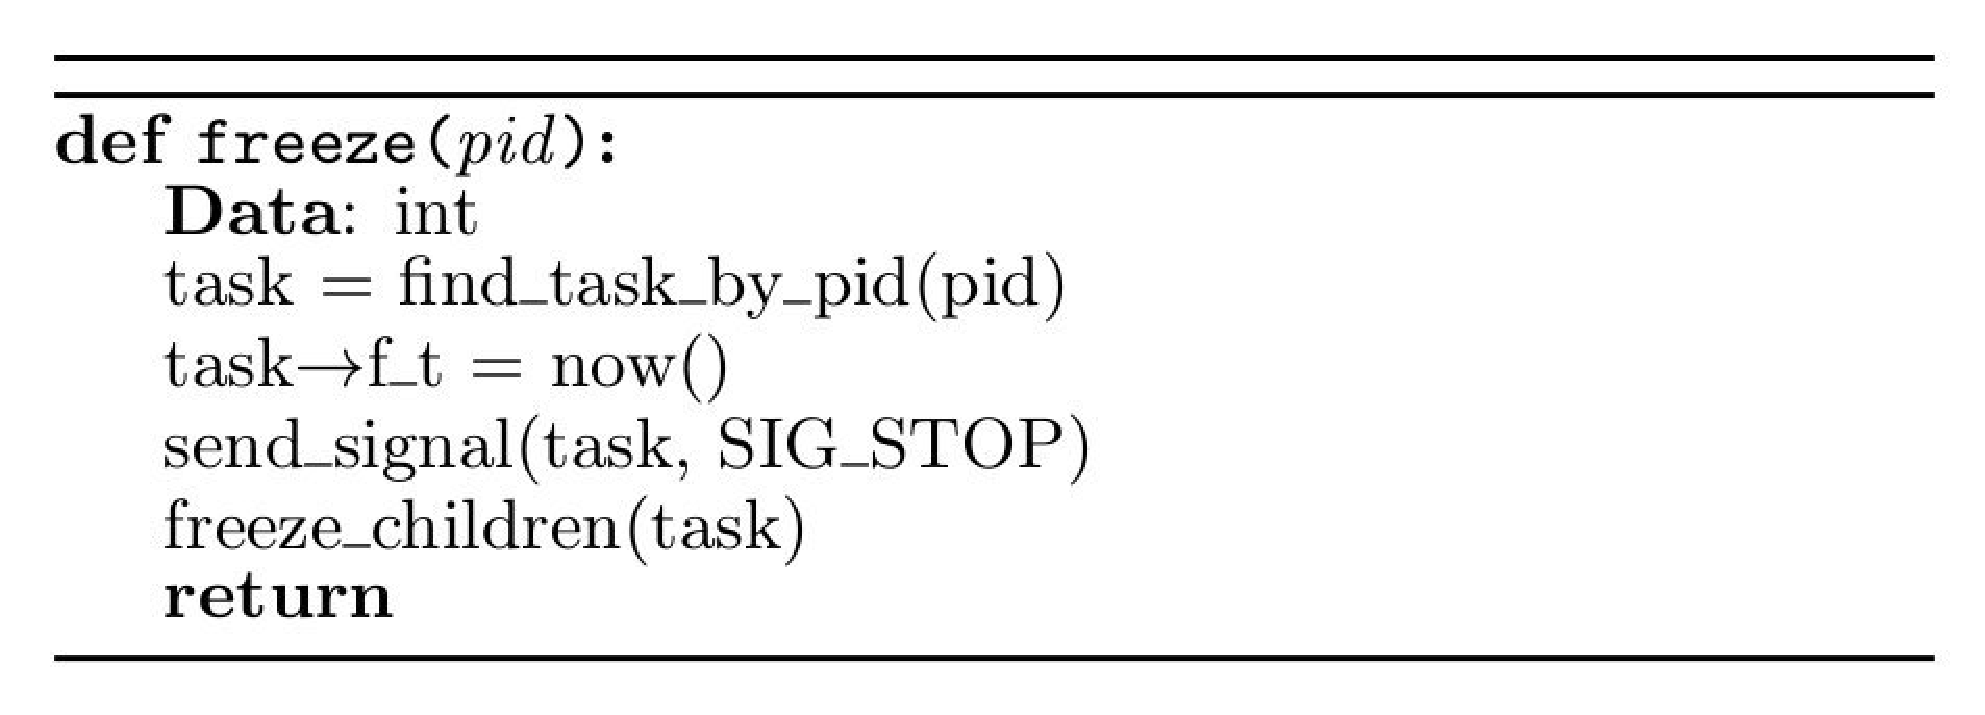
\includegraphics[width=\textwidth]{images/freeze_alg.eps} 
    \caption{Pseudocode For Freeze Functionality} 
    \label{fig:freeze_alg} 
  \end{figure} 
\begin{figure}[t] 
      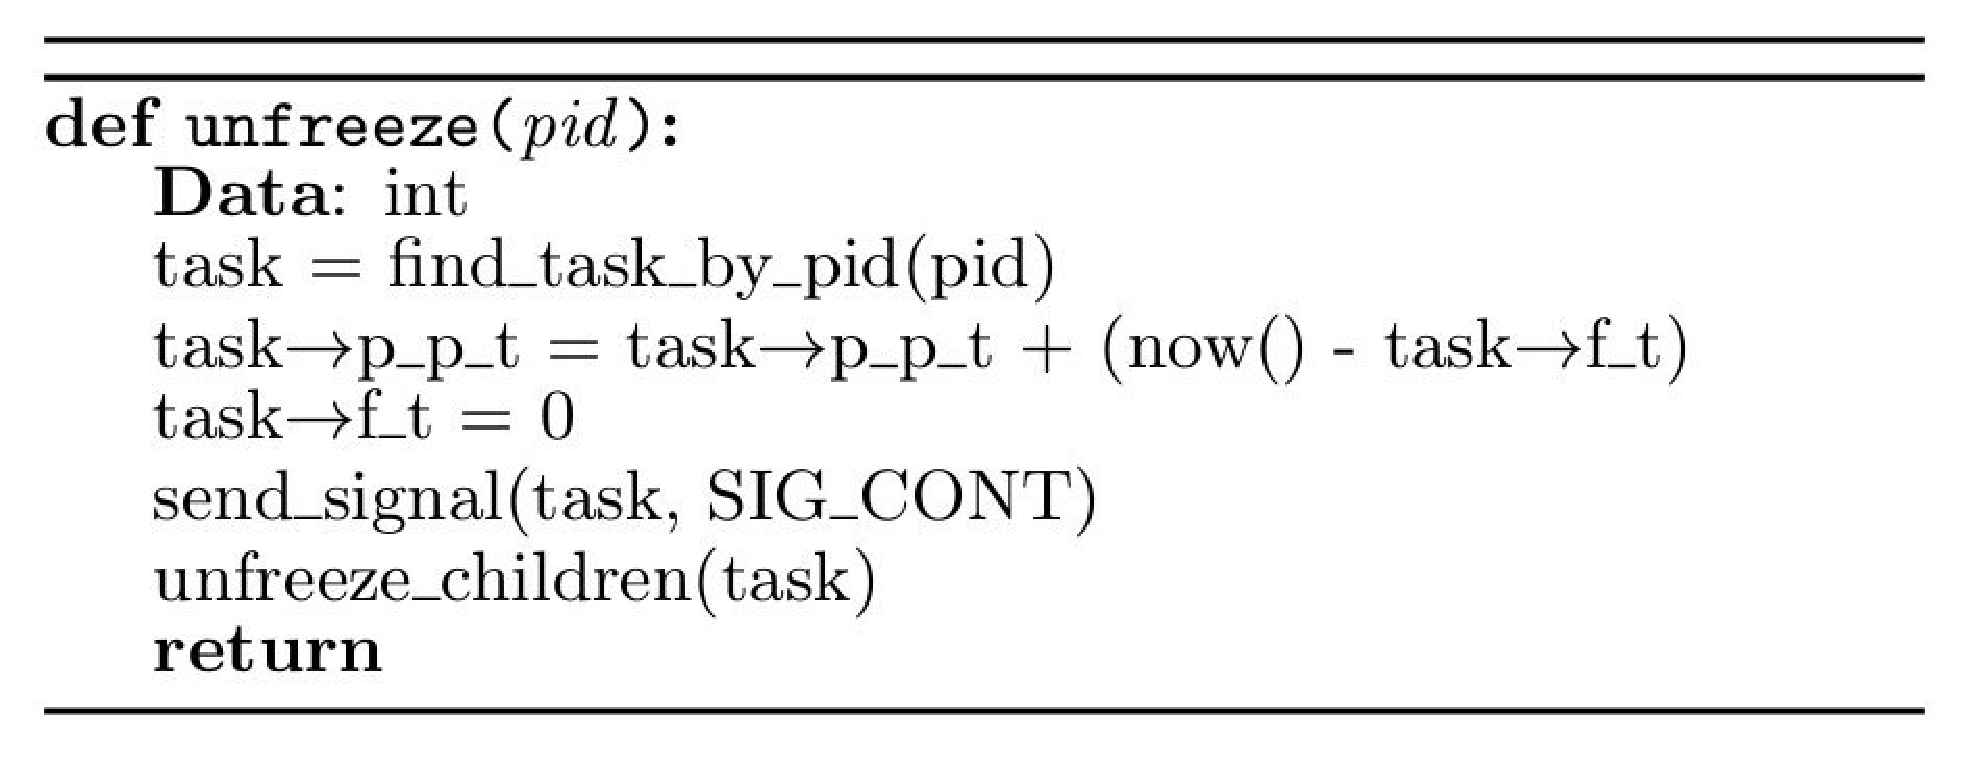
\includegraphics[width=\textwidth]{images/unfreeze_alg.eps} 
    \caption{Pseudocode For Unfreeze Functionality} 
    \label{fig:unfreeze_alg} 
  \end{figure} 
\subsection{Experiment Synchronization}
\label{subsec:experiment_synchronization}
        The TLKM is also capable of grouping processes with different TDFs together into a single $experiment$, where all of the processes virtual times progress uniformly. 
        In order to do this, TimeKeeper maintains a linked list of all processes in the experiment, an adjustable knob called $EXP\_CPU$, and another adjustable knob called a $timeslice$. $EXP\_CPU$ specifies how many processors you are willing to dedicate to the $experiment$. A higher $EXP\_CPU$ value will allow the the $experiment$ to run faster and complete in a shorter amount of physical time. A lower $EXP\_CPU$ value will make the experiment take longer to complete, but more resources will be available for other tasks. In our experiments, we would set $EXP\_CPU$ to be two processors less than the total number of processors on the system. This allows standard background tasks to still be able to run successfully, even if a CPU-intensive experiment is being conducted. The $timeslice$ variable specifies the amount of physical time in which the $leader$ process is allowed to run for each round of the experiment. When an $experiment$ is initialized, TimeKeeper will determine the $leader$, which is the process with the highest TDF. Knowing the $leader$ is a necessity, as the $leader's$ virtual time will progress slower than any other process in the experiment (because it has the highest TDF). Therefore, TimeKeeper needs to scale down the running time of all other processes in the experiment accordingly. See Table \ref{table:cpufraction} for how the $leader's$ TDF affects the running time of other processes in the experiment. 
\begin{table} \centering 
\begin{tabular}{|c|c|c|c|} 
        \hline 
         & TDF 2 & TDF 1 & TDF .5  \\ \hline 
        Leader TDF 10 & 1/5 & 1/10 &  1/20 \\ \hline 
        Leader TDF 5 &  2/5 & 1/5 & 1/10 \\ \hline 
        Leader TDF 2 & 1 & 1/2 & 1/4 \\ \hline 
        Leader TDF 1 & x &  1 & 1/2 \\ \hline 
        \hline 
        \end{tabular} 
        \caption{How Leader's TDF Affects other LXCs Fraction of CPU Time} 
        \label{table:cpufraction} 
\end{table}
For example, consider a $leader$ with a TDF of 2, and another process with a TDF of 1. In order to keep these processes' virtual times synchronized, the process with a TDF of 1 will need to run for one half the time in which the $leader$ is allowed to run. 
\begin{figure}[t] 
      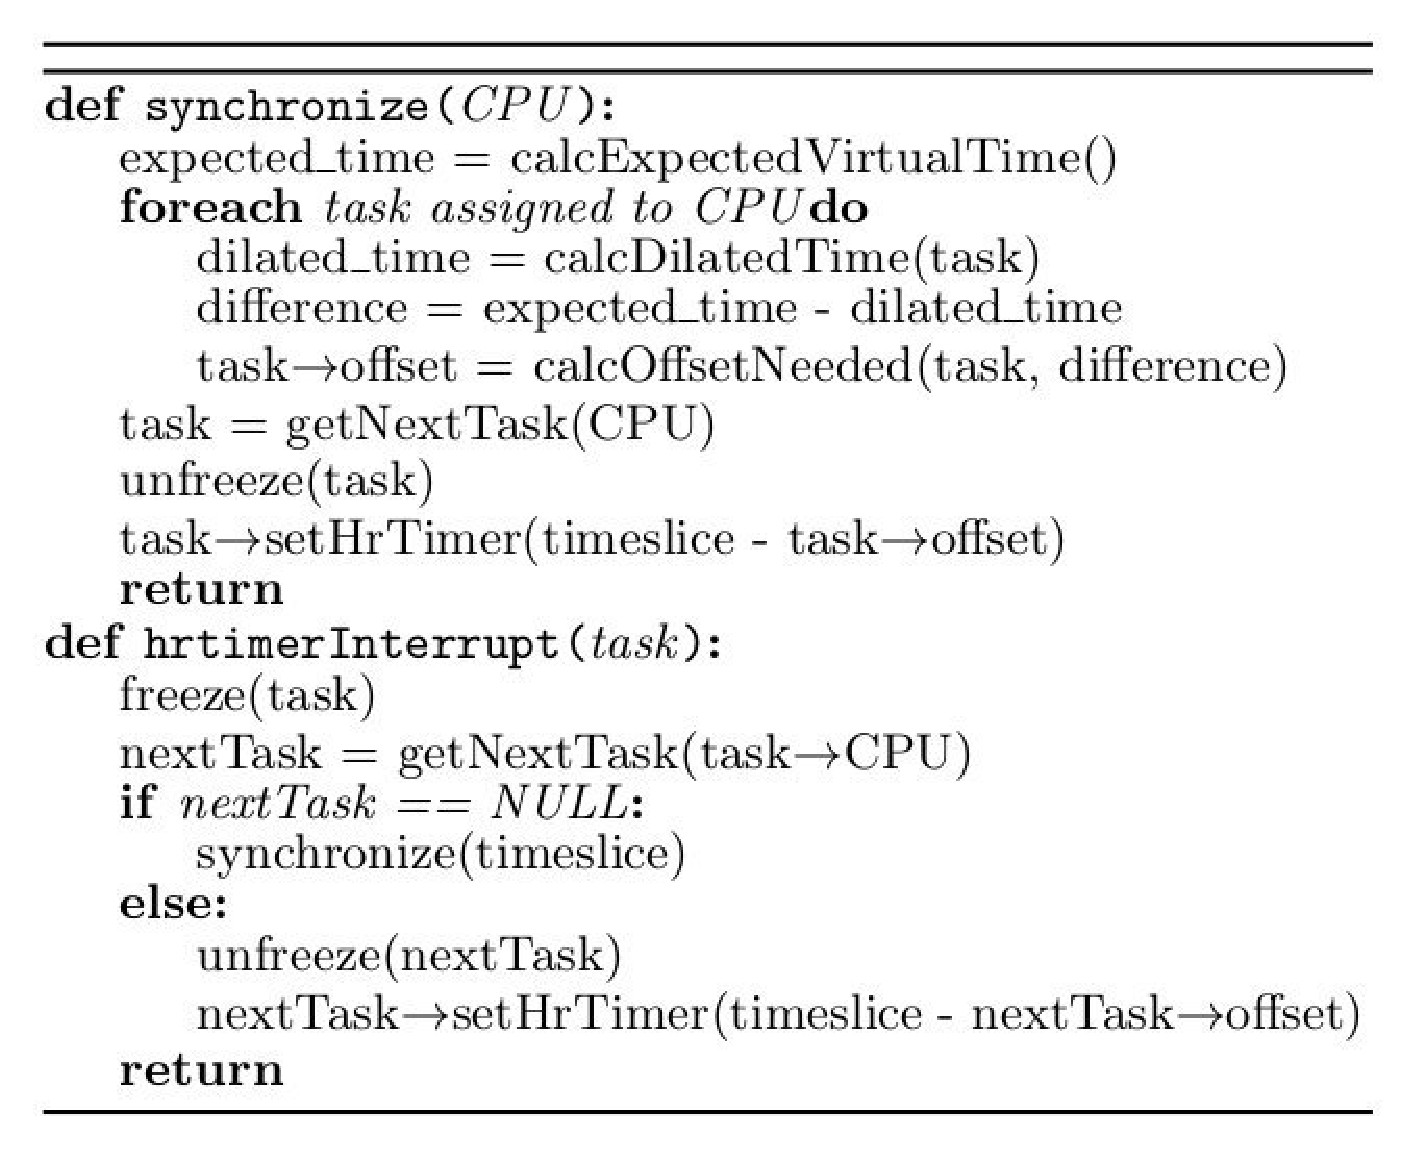
\includegraphics[width=.9\textwidth]{images/synchronization_alg.eps} 
    \caption{Pseudocode For LXC Synchronization Algorithm } 
    \label{fig:synchronization_alg} 
  \end{figure} 
        Once the $leader$ has been appointed, each process in the experiment is dedicated to a specific processor, where multiple processes may be mapped to the same processor, and set to have a scheduling policy of SCHED\_FIFO (first-in first-out). A SCHED\_FIFO scheduling policy allows the process to have a higher priority than other tasks not in the experiment, as well as not get preempted until TimeKeeper decides the process should no longer be allowed to run. Then, each process will be allocated a fraction of the $timeslice$ in which it will be allowed to run on its dedicated processor for each round. This fraction of the $timeslice$ is based on the process's TDF with respect to the $leader's$ TDF, and maintained by a high-resolution timer ($hrtimer$). At the beginning of each round of the experiment, all processes are in the $frozen$ state. For each dedicated CPU a process is chosen to run, and it is unfrozen with TimeKeeper's previously mentioned $unfreeze$ capability. When the process is unfrozen, its respective $hrtimer$ is set to expire when its predetermined fraction of the $timeslice$ is up. When the $hrtimer$ for the process expires, the process is frozen, and the next process whose turn it is to run on the CPU is unfrozen and has its $hrtimer$ set. This process continues until all processes in the $experiment$ have been allowed to run for their fraction of the $timeslice$. When all processes in the $experiment$ have ran, the round is up. At the beginning of each round, a new $leader$ may be calculated if the current $leader$ finished executing, if new processes with higher TDFs were added to the experiment, of if a process in the experiment had its TDF changed to be higher than the current $leader$. In addition, a simple check will be done for each process to determine if it should run a little longer or little less in the following round. This is done by comparing each process's virtual time to the expected virtual time of the experiment. If the process's virtual time exceeds the expected virtual time of the experiment, that process will be forced to run for less time in the current round (by setting its $hrtimer$ to fire sooner). If a process's virtual time is below the expected virtual time of the experiment, that process will be allowed to run for more time in the current round (by setting its $hrtimer$ to fire later). When all processes know how long they can run for the current round, the round may continue. See Figure \ref {fig:synchronization_alg} for the psuedocode for the synchronization algorithm.
\subsection{Hooking the System Call Table}
\label{sec:hooking}
The TLKM also needs to hook the system call table in order to ensure certain system calls like $sleep()$ behave appropriately when called from a process within a synchronized experiment. The modified $sleep()$ system call as referenced in Section \ref{sec:kernel_modifications} will work correctly if the calling process is running independently, because you can simply look at the process's TDF. However, if the calling process is within a synchronized experiment, the virtual time will be advancing at the rate of the leader's TDF, not the calling process's TDF. Therefore, the process will need to be awoken when the experiment's virtual time reaches the wake up point. To determine this point, the $sleep()$ system call is replaced dynamically with our own function when the TLKM is loaded into the Linux Kernel. The new function will first determine if the calling process is within a synchronized experiment. If it is not, it will perform the regular $sleep()$ system call. If the process is within a synchronized experiment, it will be put to sleep, and set to resume execution when the experiment's virtual time surpasses the wake up time. When the TimeKeeper Kernel Module is removed from the Linux Kernel, the $sleep()$ system call is unhooked and returned to its regular functionality.

\section{CORE Integration}
CORE is capable of emulating the networking stack of various routers and end hosts through virtualization and then simulating the links between such devices. CORE was chosen as the initial system to be integrated with TimeKeeper because it uses network namespaces to divide processes into logically separate networking entities (giving each process its own routing tables, network adapters, and so forth). Internally, LXCs use network namespaces to achieve the same goal. However, LXCs provide additional features, such as the ability to create persistent containers via configuration files, or resource isolation via cgroups. CORE does not need the advanced features of LXCs, so the simpler network namespace alternative was used. Because LXCs are so closely tied to network namespaces, it made CORE an ideal first system to integrate with TimeKeeper. The next two sections will give an overview of how CORE works under the hood, followed by a description of the necessary changes made for the TimeKeeper integration. 
\subsection{CORE Subsystem Overview}
CORE consists of two major components: a Tcl/Tk GUI frontend, and a CORE daemon backend. The CORE daemon listens on a local TCP port for specific messages (known as the CORE API) from the graphical user interface (GUI), giving it commands to create specific topologies. To help illustrate what is going on behind the scenes, I will use a simple 2-node example as shown in Figure \ref{fig:core2node}. 
\begin{figure}[t] 
      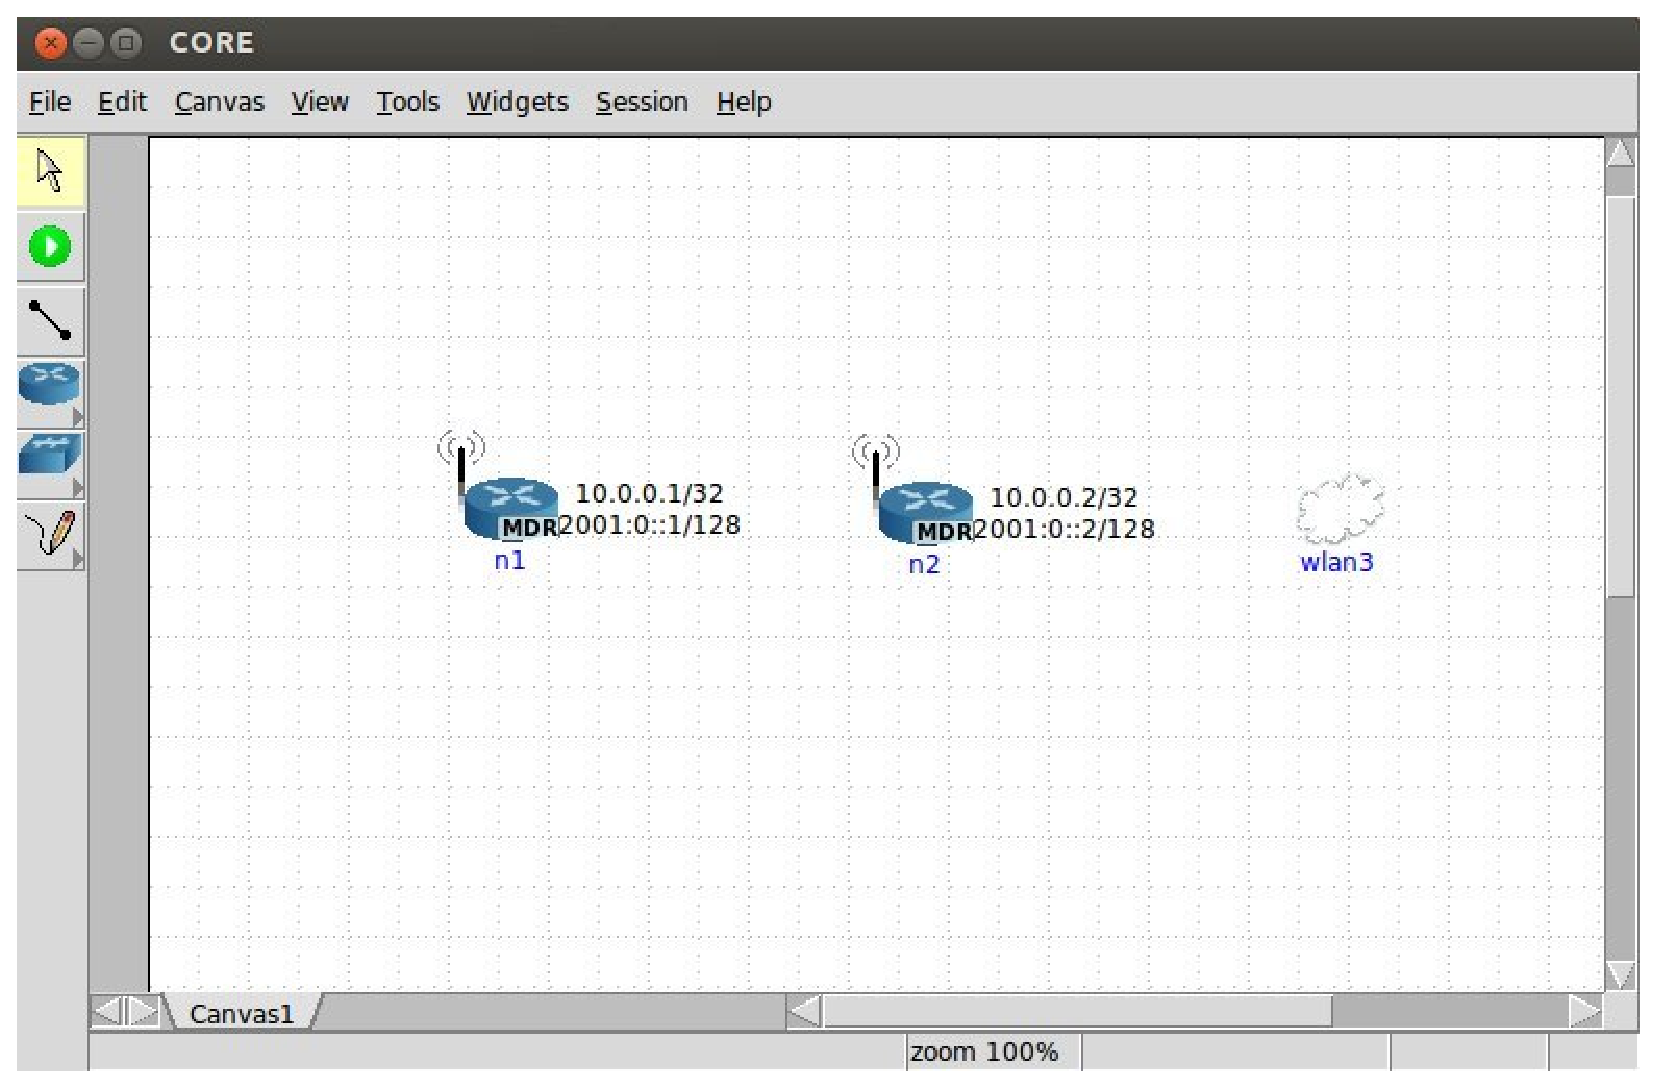
\includegraphics[width=\textwidth]{images/core2node.eps} 
    \caption{Simple 2-Node Topology in CORE} 
    \label{fig:core2node} 
  \end{figure}
This example will model basic on/off wireless connectivity. If the two routers are close enough (as determined by the physical distance from one another in the CORE GUI), they will be able to communicate, if the routers are too far away they will not be able to communicate. The experiment will be started when the green play button is clicked from within the GUI. When this action occurs, the GUI will send all necessary messages describing the created topology to the CORE daemon. For every node in the topology (router or host), the GUI will send a $Node Message$ to the CORE daemon, which will spawn a $vnoded$ daemon responsible for creating its own network namespace. To establish the connectivity, CORE will use a combination of virtual Ethernet pair drivers ($veth$), Linux Bridging, and Ethernet Bridging Tables (ebtables). A $veth$ is simply a Ethernet-like device that can be used inside of a container. Each $veth$ consists of two Ethernet devices, one of which will be installed on the host, while the other will be installed inside the newly created container. When a packet is sent to one of the devices, it will simply come out the other device. The appropriate $veth's$ will then be tied together with Linux bridges. You may think of a Linux bridge as a switch. Finally, appropriate $ebtable$ rules will be applied to the bridge, determining if packets should be dropped or not, depending on the physical distance between the containers. See Figure \ref{fig:coreInternals} to see how two containers are connected in CORE.
\begin{figure}[t] 
      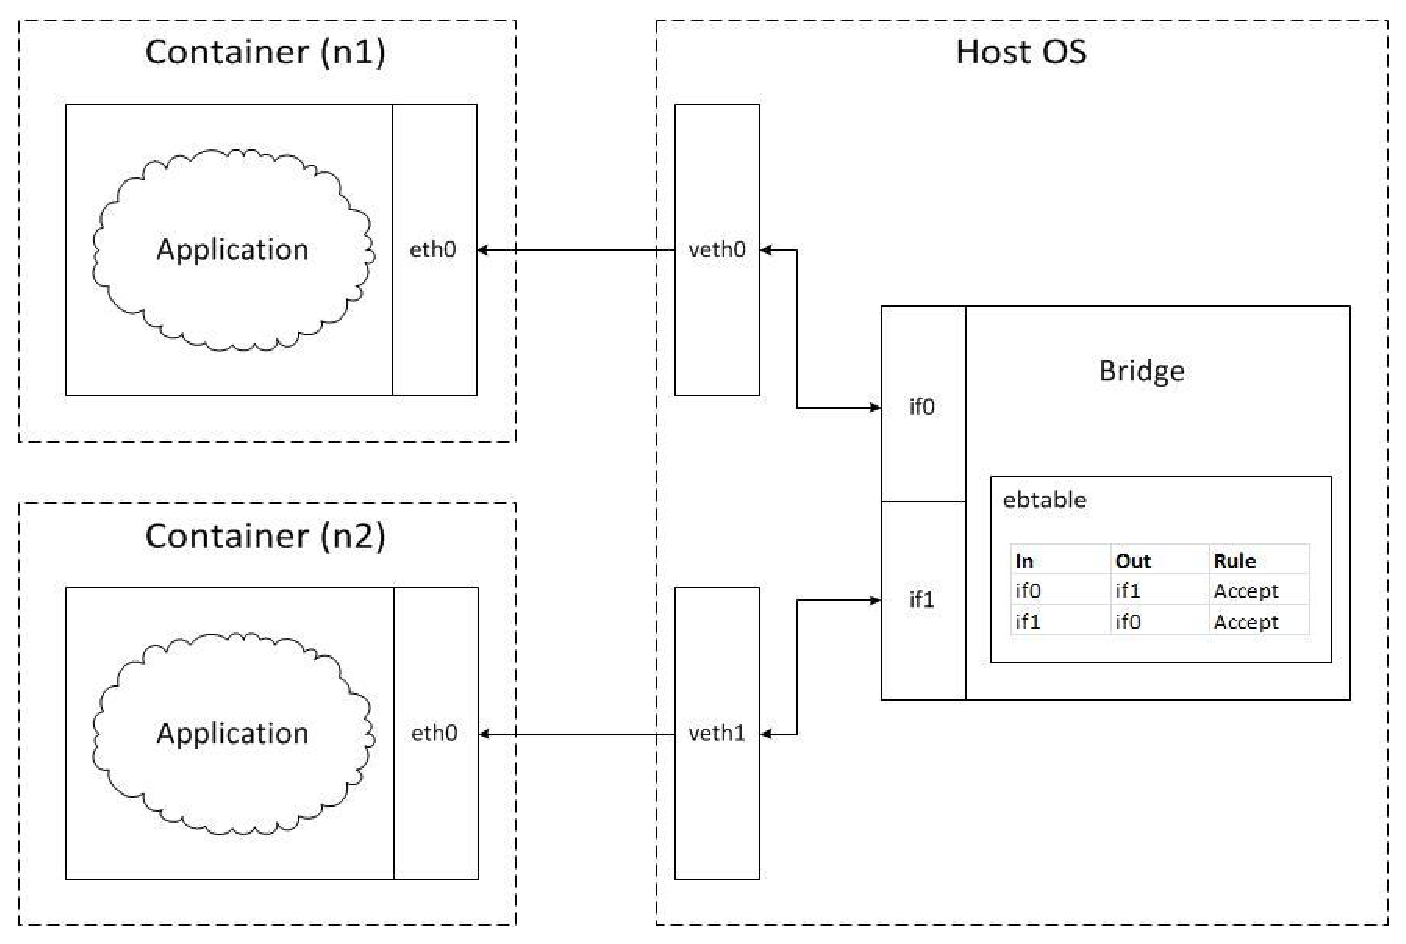
\includegraphics[width=\textwidth]{images/coreInternals.eps} 
    \caption{Connecting Two Containers Within CORE} 
    \label{fig:coreInternals} 
  \end{figure}
\subsection{CORE Modifications}
In order to integrate TimeKeeper with CORE, only a few changes had to be made. Modifications had to be made to allow both the GUI and $vnoded$ daemon to communicate with TimeKeeper. These modifications are illustrated below, and accompanied with a flowchart depicting the changes (see Figure \ref{fig:coreContainerCreation}). 
\begin{enumerate}
        \item First, the GUI was modified in order to maintain additional topology information, and provide the means for the user to input additional information. Now, if a user double clicks on a entity, the option is provided to set that entities TDF. Alternatively, the user could set the TDF of every entity in the window from the 'Tools' tab. The GUI maintains state information for every entity in the window, so when the TDF is set for an entity, its corresponding dilation variable is set appropriately. 
        \item When the topology is constructed, the user clicks the green play button to start the experiment. When this button is clicked, one thing the GUI will do is traverse $node\_list$, which is a list of every node in the GUI. For every node, a “Node Message” which contains information for that node will be sent to CORE daemon. The “Node Message” contains a field called 'opaque' which is meant for user-defined data. Each entities TDF is passed to the CORE daemon via this 'opaque' field.
        \item The CORE daemon receives each “Node Message”, and handles it with the $handlenodemsg$ function. The function extracts the necessary information from the “Node Message”, including the TDF. Then, a modified $vnoded$ script is called. This modified script is able to accept an additional command line argument, the TDF of the container.
        \item The $vnoded$ script calls $nsfork$, which actually creates the network namespace via a $clone()$ system call. The $nsfork$ function was modified so once the $clone()$ system call returns, the new container immediately gets assigned its TDF. Before $nsfork$ returns, it sends the PID of the new container to TimeKeeper. This tells TimeKeeper to add the new container to the synchronized experiment. 
        \item After a short time, all of the time-dilated containers will be set up, and the CORE experiment will begin. From this point, the user may tell TimeKeeper to start the experiment in order to have all the containers virtual time progress uniformly through time. This can be done through the 'Tools' tab, which will send the start message to TimeKeeper. 
\end{enumerate}

\begin{figure}[t] 
      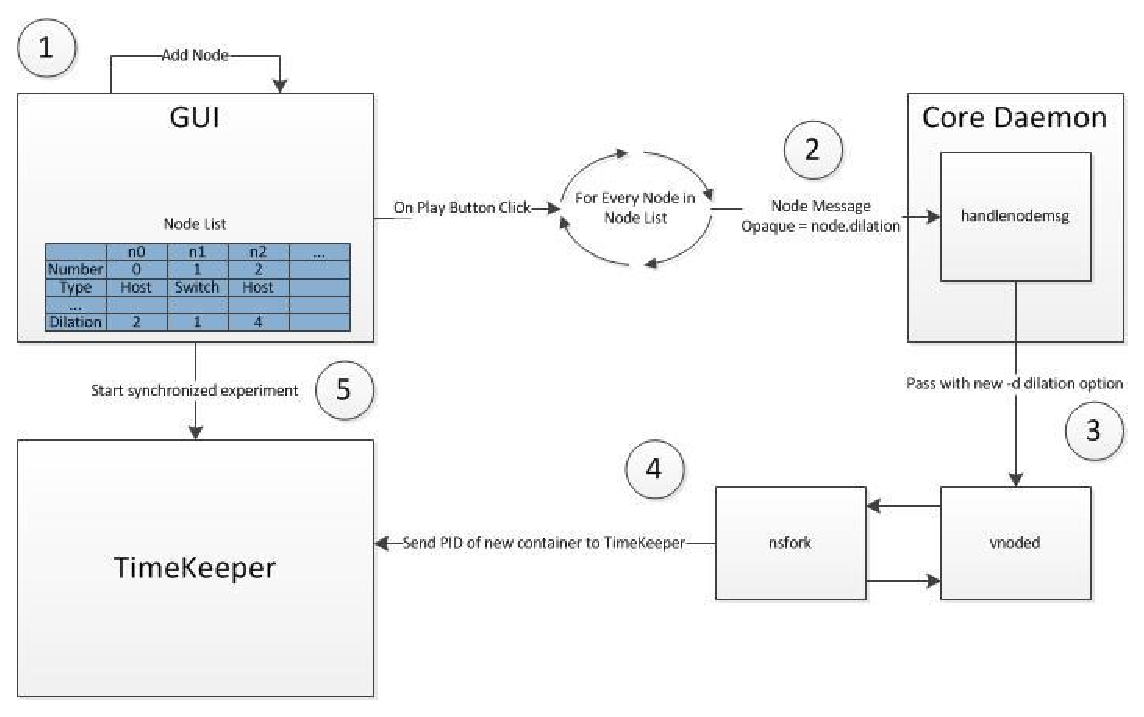
\includegraphics[width=\textwidth]{images/coreContainerCreation.eps} 
    \caption{Core Modifications To Support TimeKeeper} 
    \label{fig:coreContainerCreation} 
  \end{figure}

\section{NS-3 Integration}
NS-3 is an extremely popular discrete-event network simulator, designed primarily for research or educational use. It is composed of numerous 'network' models, such as Wi-Fi or LANs. We are particularly interested in ns-3's ability to interact with real systems, for 'simulation-in-the-loop' experiments. This is done with a RealTime Scheduler. The following two sections will give a brief overview of how ns-3 works under the hood, followed by a description of the necessary changes made for TimeKeeper integration. 
\subsection{NS-3 Subsystem Overview}
Describing all of the components composing ns-3 would be out of the scope of this paper. Instead, we will focus on the components that allow us to hook LXCs to the ns-3 simulator: the RealTime Scheduler and the TapBridge Model. The will be discussed separately.
\begin{itemize} 
                        \item \textbf{RealTime Scheduler} \\ 
                        The default scheduler for ns-3 is not realtime. In this case, when an event is processed, the simulator's time will jump to the time of the next scheduled event. Obviously, this technique will not work if ns-3 is tied to an external entity, as it may send a network packet at any time. If the simulation clock is jumping far ahead, it will not process this packet correctly. Thus, the RealTime Scheduler was implemented, which attempts to keep ns-3's simulation clock synchronized with respect to an external time base (most commonly the wall clock). The RealTime Scheduler works as follows: When the next event in the simulation is ready to be processed, the scheduler will compare the system clock with the scheduled time of the event. If the scheduled time of the event is close to the system clock, it will get executed. If the scheduled time of the event is in the future, the simulator will sleep until the system clock catches up to the scheduled time of the event, then execute that event. It is also possible for the simulator to fall behind the system clock (if the simulator can not process a series of events fast enough). For when this happens, the scheduler has two options, which the user can specify: BestEffort or HardLimit. If the scheduler is running in BestEffort, it will repeatedly process events until it is able to catch up to the system clock. It may never be able to catch up to the system clock if the simulator is constantly overloaded with events. The HardLimit option will also try to catch up to the system clock, but will end the simulation if the difference between the system clock and the simulation clock becomes too large. See Figure \ref{fig:realtimeScheduler}.

\begin{figure}[t] 
      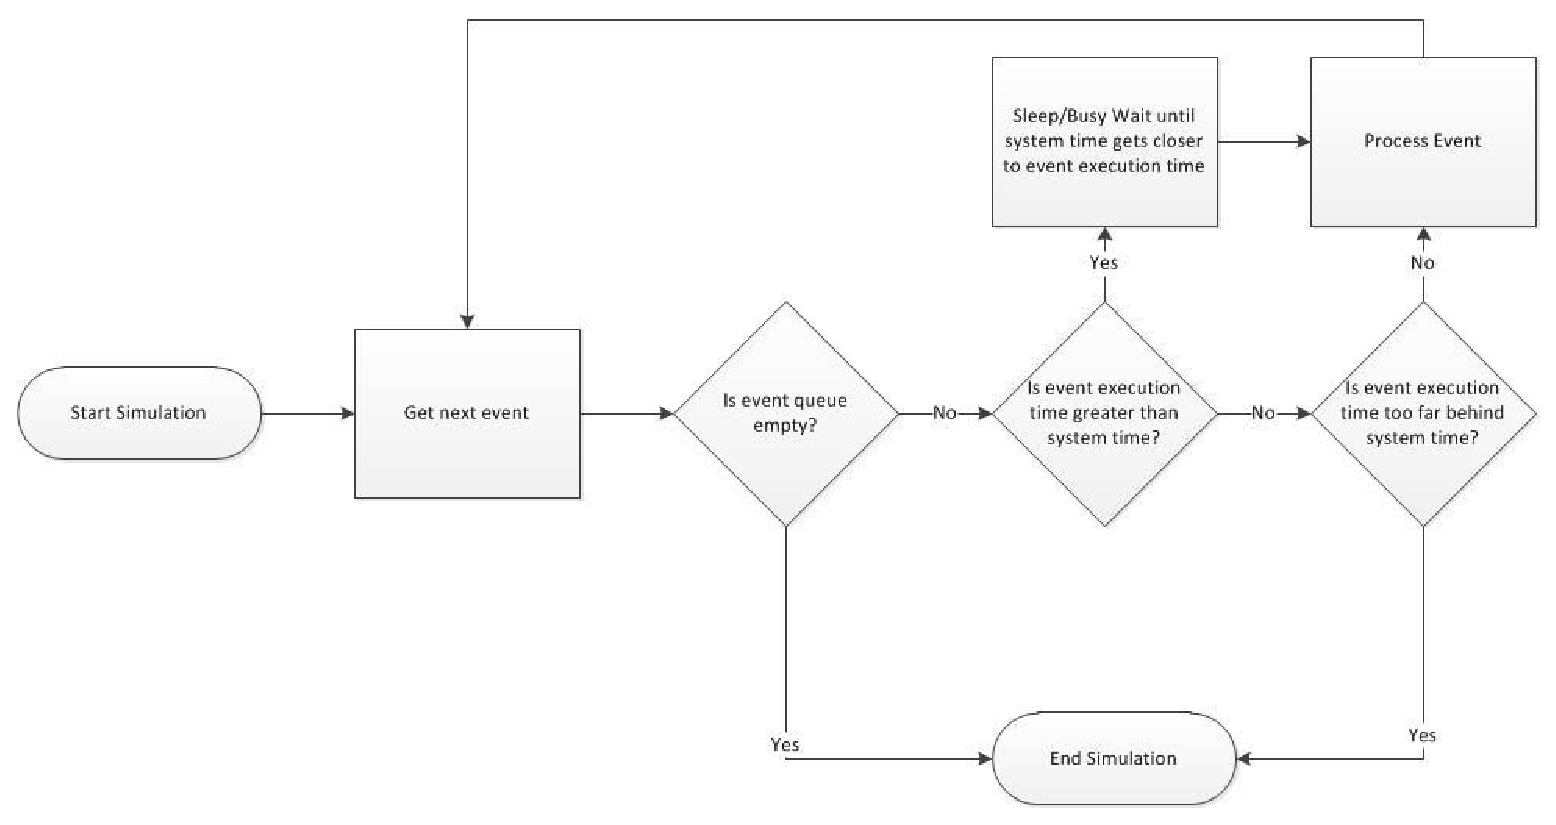
\includegraphics[width=\textwidth]{images/realtimeScheduler.eps} 
    \caption{Simplified NS-3 Flowchart with Realtime Scheduler} 
    \label{fig:realtimeScheduler} 
  \end{figure}
                \item \textbf{TapBridge Model} \\ 
                        The TapBridge Model was designed to integrate real internet hosts (LXCs) with an ns-3 simulation. It works by essentially connecting the inputs and outputs of a Linux TAP device with the inputs and outputs of an ns-3 Net Device. A Linux TAP device allows for user space programs to send and receive packets without needing to traverse physical media. The Linux TAP acts as the glue connecting an LXC and the ns-3 simulation. In ns-3, the Net Device is an abstraction which covers the simulated hardware as well as the software driver. It can be installed on a 'Node', which enables the Node to communicate with others in the simulation. For every real internet host (or LXC) we wish to integrate into the ns-3 simulation, the TapBridge Model will create a 'Ghost Node'. A Ghost Node is simply a Node that is representing an external entity (where the upper levels are not being simulated). For every TapBridge on the Ghost Node there is a corresponding ns-3 NetDevice in which it is acting as the bridge. Everytime the LXC sends a packet, the TAP Device will bring it into user-space, modify the MAC addresses appropriately, and forward it to the Net Device. Likewise, when a packet is received on a ns-3 NetDevice, the TapBridge will grab it, modify the MAC addresses, and send it out the TAP Device. The MAC addresses within packets need to be modified because the TAP Device and ns-3 NetDevice have different MAC addresses. This MAC address spoofing will make it appear for the LXC to have the ns-3 NetDevice as a local device. See Figure \ref{fig:ns3internals} for how LXCs are connected to ns-3.
\begin{figure}[t] 
      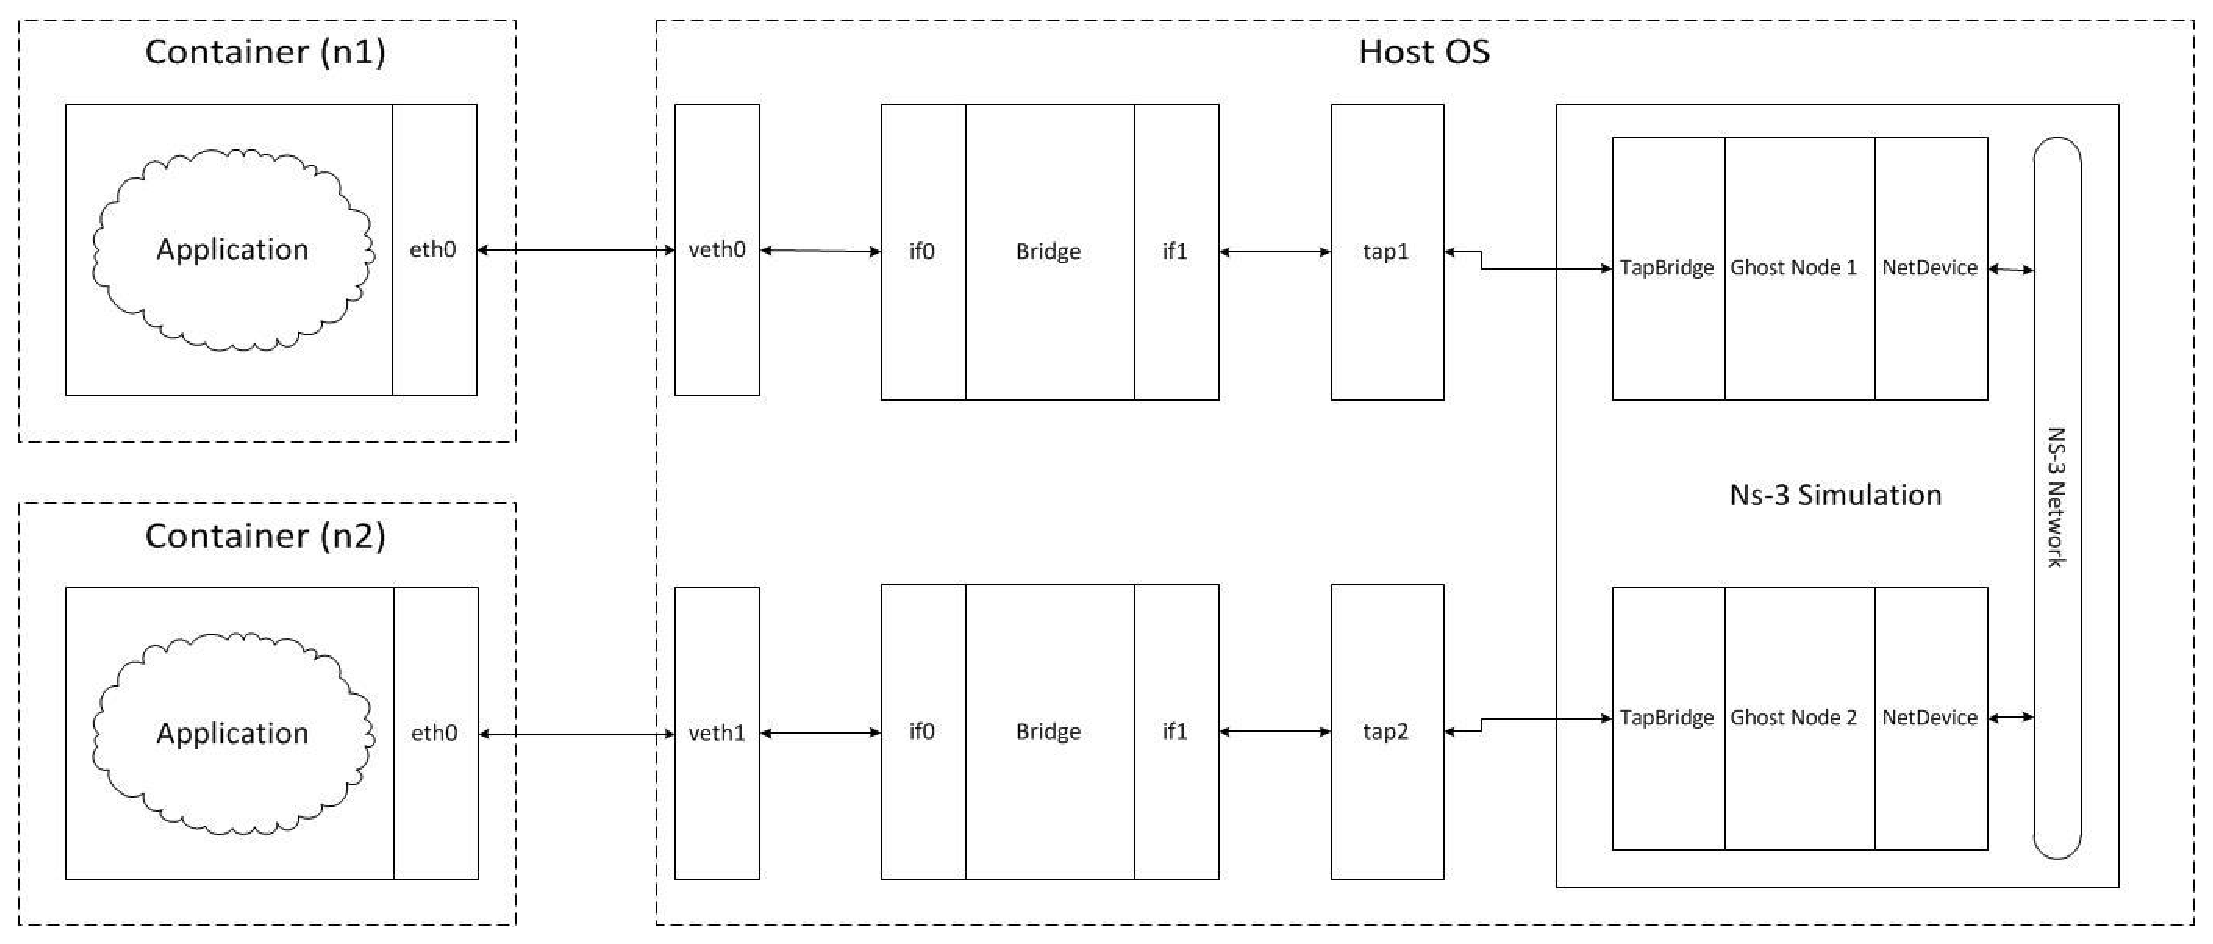
\includegraphics[width=\textwidth]{images/ns3internals.eps} 
    \caption{Connecting LXCs to ns-3} 
    \label{fig:ns3internals}
  \end{figure}
        \end{itemize}
\subsection{NS-3 Modifications}
Integrating TimeKeeper with ns-3 was actually surprising simple. In fact, no changes needed to be made to the ns-3 source code to allow for integration with TimeKeeper! This is because the ns-3 simulator is simply a process with a number of threads. In addition, the RealTime Scheduler utilizes the $gettimeofday()$ system call to determine how far away the simulation time is from the system time. Therefore,  all that is necessary is to add the ns-3 process to the synchronized experiment and assign it a TDF. Then, ns-3's notion of simulation time will progress at the same rate as the other LXCs in the experiment, keeping all of the virtual times synchronized.

\chapter{Evaluation} 
\label{chap:experiments}
Unless otherwise specified, the following experiments were conducted on a Dell Studio XPS Desktop, with 24 GB of RAM, and 8 Intel Core i-7 CPU X 980's @ 3.33GHz. The machine is running either 32-bit or 64-bit Ubuntu with the modified 3.10.9 Linux Kernel.

\section{Hrtimer Accuracy}
\label{sec:hrtimer}
The effectiveness of TimeKeeper's ability to keep virtual clocks synchronized is highly dependent on the $hrtimer's$ ability to fire interrupts at precise moments in time. For example, if we need a particular LXC to run for 1$\mu s$ at a time, then we would want the $hrtimer$ associated with that particular LXC to trigger an interrupt as close to 1$\mu s$ as possible. For the initial test, we set different $hrtimers$ to periodically fire at different time intervals ($timeslice$), and measured what time the $hrtimer$ interrupt actually fired. We collected 200 data points for every different time interval. From there, we calculated the mean ($\mu$) and standard deviation ($\sigma$) of the error. Table \ref{table:hrtimerAccuracy} presents the results.

\begin{table}\centering 
\begin{tabular}{|c|c|c|c|} 
        \hline 
        timeslice & $\mu$ & $\sigma$ \\ \hline 
        300$ms$ & 862ns &  1130ns \\ \hline 
        30$ms$ & 401ns &  680ns \\ \hline 
        3$ms$ & 341ns&  592ns \\ \hline 
        300$\mu s$ & 523ns &  2306ns \\ \hline 
        30$\mu s$ & 351ns &  2128 ns\\ \hline 
        3$\mu s$ & 481ns &  3312ns \\ \hline 
        1$\mu s$ & 2404ns &  4213ns \\ \hline 
        300$ns$ & 2925ns  & 6012ns \\ \hline 
        \hline 
        \end{tabular} 
        \caption{Mean and Standard Deviation of Timer Error for Different Timeslice Lengths} 
        \label{table:hrtimerAccuracy} 
\end{table}

Taking the first row as an example, when the timer was scheduled to fire an interrupt every 300$ms$, on average the interrupt occurred 862$ns$ from what was expected.  This is excellent accuracy, there are five orders of magnitude between the error and the $timeslice$. The magnitude of the variation in error is roughly constant; the error size relative to $timeslice$ is still an order of magnitude smaller with a 30 micro-second $timeslice$, and is roughly equal with a 3 micro-second $timeslice$.  These comparisons tell us something very important about the level of granularity we can effectively use in combined emulation/simulation scenarios.  If 10\% error in timing is acceptable and a simulated message takes on the order of 100 micro-seconds to pass on the network from one device to 
another, we can expect to get a little over three $timeslices$ in during the message's passage 
through the network simulator. {\em This} means that if a container is sensitive to IO from the simulator only at $timeslice$ boundaries (as is the case with the virtual-time OpenVZ system), there may be as much as a 33\% error in the virtual time at which the container ``sees" the message.    The take-away message here is that Linux timers are very accurate, but if we are to be able to take advantage of that accuracy when interfacing emulated LXC containers and a network simulator we will have to find a way to integrate simulator time and container time at a finer granularity than the $timeslice$.  This constitutes one of our areas of future work.

\section{Synchronization}
To integrate our emulation with network simulation we will need to keep LXCs closely synchronized.  We performed a set of experiments to evaluate how tightly we are able to do so. 
\subsection{Synchronized Experiment Accuracy}
In these experiments, TimeKeeper aimed to have each LXC achieve a target virtual time by the end of each $timeslice$. For each LXC and each $timeslice$ we measure the deviation of the virtual time the LXC actually achieved at that $timeslice$ from the target goal.  For each set of experiments we compute the mean error $\mu$ and the the standard deviation of the error $\sigma$, taken over all LXCs and synchronizations, and observe the behavior of these errors as a function of the number of LXCs and the size of the $timeslice$.  Our first round of experiments used the same TDF for all containers; 
each container was engaged in the compute-intensive task of computing the factorial of a large number.

\begin{table}\centering 
\begin{tabular}{|c|c|c|c|c|} 
        \hline 
       \# of LXCs & timeslice & $\mu$ & $\sigma$ \\ \hline 
        10 & .3ms & 596ns & 1084ns \\ \hline 
        10 & 3ms & 685ns & 1129ns \\ \hline 
        10 & 30ms & 1028ns & 1766ns \\ \hline 
        10 & 300ms & 812ns & 1447ns \\ \hline 
        80 & .3ms & 196ns & 375ns \\ \hline 
        80 & 3ms & 193ns & 374ns \\ \hline 
        80 & 30ms & 258ns & 535ns \\ \hline 
        80 & 300ms & 333ns & 628ns \\ \hline 
        \hline 
        \end{tabular} 
        \caption{Mean and Standard Deviation of Error as a Function of Timeslice and \#LXCs} 
        \label{table:msesamedil} 
\end{table}

For the first experiment, we used a TDF of 10 for each container, and recorded measurements for 150 $timeslice$ intervals. The results are summarized in Table \ref{table:msesamedil}, and reveal some interesting information. First, it demonstrates that TimeKeeper is effective at keeping virtual times synchronized on the $timeslice$ sizes used. TimeKeeper is seemingly more effective at keeping the experiment synchronized when the $timeslice$ length is 3$ms$ rather than 300$ms$. At the time of this writing we are unsure of the underlying cause for this difference, and are working at additional 
instrumentation in an effort to uncover an understandable explanation.

\begin{figure} \centering  
      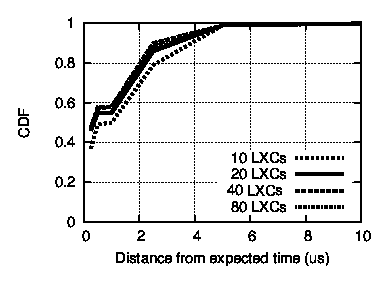
\includegraphics[width=0.8\textwidth]{images/cdf_3ms_xnodes.eps} 
    \caption{CDF with timeslice=3ms as a function of \#LXCs} 
    \label{fig:sync1} 
  \end{figure} 

\begin{figure} \centering 
      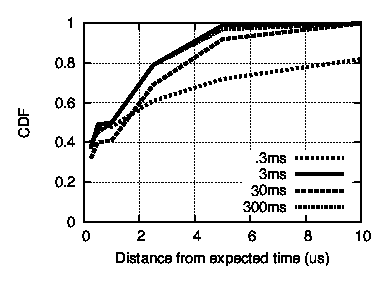
\includegraphics[width=0.8\textwidth]{images/cdf_xms_10nodes.eps} 
    \caption{CDF with 10 LXCs as a function of timeslice length} 
    \label{fig:sync2} 
  \end{figure}

To give better insight into the distribution of error, we also plotted two cumulative distribution functions (CDFs). Figure \ref{fig:sync1} shows us a CDF when the number of LXCs in the experiment range from 10-80, and the $timeslice$ interval is constant at 3$ms$. Regardless of whether the experiment had 10 LXCs or 80 LXCs, TimeKeeper was able to keep every LXCs virtual time within 4$\mu s$ of the expected virtual time for more than 90\% of each $timeslice$ interval. However, this comes at a cost. The more LXCs you add to the experiment, the longer it takes for the experiment virtual time to progress. This will be explored more fully in Section \ref{sec:over}. Figure \ref{fig:sync2} shows us a CDF when we have an experiment size of 10 LXCs (where 5 LXCs have a TDF of 10, and 5 LXCs have a TDF of 1), and we vary the $timeslice$ interval lengths. In general, TimeKeeper is able to keep the experiment virtual time in sync, but we noticed when the $timeslice$ interval is .3$ms$ that it did not perform as well. These results correspond with what we found in Table \ref{table:hrtimerAccuracy} (where the $hrtimers$ were not as accurate at a granularity of .3$ms$ as opposed to higher granularities).

\subsection{Scalability}

Figure \ref{fig:scale} demonstrates scalability, plotting how the mean and standard deviation of the error behaves as the number of containers grows.  Again we see the interesting phenomena that the error decreases with increasing numbers of containers;  the error is also contained almost always to be less than half a micro-second. 

\begin{figure} \centering
      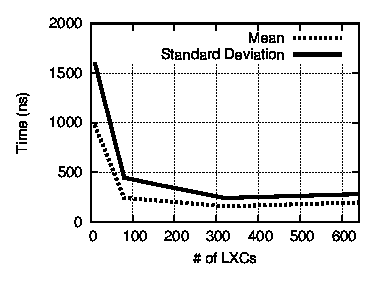
\includegraphics[width=0.8\textwidth]{images/scale.eps} 
    \caption{Testing Scalability with a Timeslice of 3ms and a TDF of 1/10} 
    \label{fig:scale} 
  \end{figure} 

We obtained access to a larger machine, with 32 cores and 64Gb of memory. This allowed us to stress test TimeKeeper and observe how many containers we can sustain.  We successfully did one experiment using 45,000 containers, which represents two orders magnitude increase of what could be done on that same machine with openVZ containers. 

We performed an experiment aimed at measuring the mean and standard deviation of the time error found when TimeKeeper tries to keep all LXC containers in an experiment synchronized. For this we keep the product of number of containers with the TDF constant, at approximately 20. The intuition is we are trying to keep the rate (in wallclock time) at which virtual time advances in the system as a whole constant---increasing the number of containers means the number of times a container is given service per unit wallclock time decreases, so each time it gets service it has to advance simulation time farther. Now in these experiments the $timeslice$ length is kept constant. 

\begin{figure} \centering 
      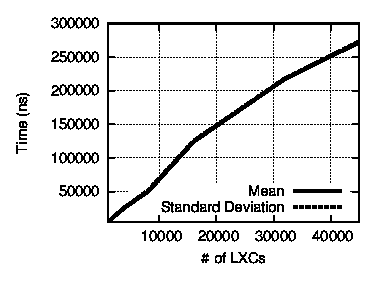
\includegraphics[width=0.8\textwidth]{images/mean_dev_large.eps} 
    \caption{Testing Scalability with the Product of \#LXCs and TDF Constant } 
    \label{fig:lxc_tdf_constant} 
  \end{figure} 

Figure \ref{fig:lxc_tdf_constant} displays the results, and reveals an interesting consequence of the scaling we employ. As the number of LXCs increases, the TDF decreases, which means that the advance in virtual time per unit wall-clock tick increases.  The error of timers {\em in wall-clock time} is unaffected by the number of containers, however this fixed error is {\em amplified} by the amplification of virtual time advancement.  This explains the linear increase in error.  We'd get essentially the same curve---but with different y-axis values---by using a different constant product of TDF and \#LXCs.  A product that is larger by a factor of 10 will yield errors that are a factor of 10 smaller.   Two main points should be appreciated from this data. One, that TimeKeeper has managed as many as 45,000 synchronized containers on a commodity server, and second, that the error of timers in real-time has more impact on the errors in virtual time the faster the containers are accelerated through virtual time.

\subsection{CS Accuracy}
In order to support CS, TimeKeeper needs to advance an LXC's virtual time by the amount specified by the user. Here, we explore how accurate TimeKeeper is at allowing a particular LXC to run to a specific period of time, then ensure it holds true when we scale the experiment to thousands of LXCs. For the experiment, we specified how long each LXC should be able to run by a static interval. Then we progressed each LXC by that interval, and calculated how far away the LXC's virtual time was from the expected virtual time. We collected 100 data points for each experiment, and modified either the interval in which the LXC's virtual time should advance at, or the number of LXCs in the experiment. The results can be found in Table \ref{table:cs_accuracy}.
\begin{table}\centering 
\begin{tabular}{|c|c|c|c|c|} 
        \hline 
       \# of LXCs & 10$\mu s$ & 100$\mu s$  & 1000$\mu s$  \\ \hline 
        8 & 2.05$\mu s$ & 9.79$\mu s$ & 67.2$\mu s$ \\ \hline 
        80 & 1.45$\mu s$ & 11.7$\mu s$ & 66.3$\mu s$ \\ \hline 
        800 & 1.88$\mu s$ & 12.13$\mu s$ & 63.5$\mu s$ \\ \hline 
        8000 & 2.0$\mu s$ & 9.34$\mu s$ & 66.9$\mu s$ \\ \hline 
        \hline 
        \end{tabular} 
        \caption{Average Error as a Function of the Virtual Time Advancement Interval and Number of LXCs} 
        \label{table:cs_accuracy}
\end{table}
The table suggests TimeKeeper is efficient at accurately maintaining the virtual times of LXCs via the CS method, regardless of the size of the experiment. With a 10$\mu s$ advancement interval, TimeKeeper was able to keep the error to within about 2$\mu s$. Another noticeable pattern is TimeKeeper appears to become more accurate as the advancement interval gets smaller. However, when the advancement interval gets too small, TimeKeeper actually becomes less accurate. This supports what we found in Section \ref{sec:hrtimer}. For example, when the advancement interval was 1$\mu s$, the average error was 6.24$\mu s$! 

\section{Overhead}
\label{sec:over}
For overhead experiments, we looked at two main areas. First, we look at how modifications to the kernel code affected the running time of the corresponding system calls. Next, we look at the overhead TimeKeeper introduces when it attempts to keep container's virtual times synchronized.
\subsection{Gettimeofday() Overhead}
The $gettimeofday()$ system call was the most heavily modified piece of kernel code, so we wanted to determine the level of impact these modifications have with respect to execution time. To test this, we created a process that would repeatedly call the $gettimeofday()$ system call with the normal Linux Kernel, measure how long each call would take, and calculate the average. Only the time spent executing the Kernel code was measured, the time spent switching from user-space to kernel-space was not measured.The experiment was repeated, but on our modified Linux kernel, and with TDF's of 1, .5, and 2. The results are summarized in Table \ref{table:gtodOverhead}.

\begin{table} \centering 
\begin{tabular}{|c|c|c|c|c|} 
        \hline 
         & Time ($ns$) & Difference ($ns$) & \% Longer \\ \hline 
        Unmodified Linux Kernel & 85.9 & 0 &  0 \\ \hline 
        Modified Linux Kernel, TDF 1 &  88.2 & 2.3 & 3 \\ \hline 
        Modified Linux Kernel, TDF .5 & 134.8 & 48.9 & 57 \\ \hline 
        Modified Linux Kernel, TDF 2 & 139.4 &  53.5 & 62 \\ \hline 
        \hline 
        \end{tabular} 
        \caption{Gettimeofday() Overhead} 
        \label{table:gtodOverhead} 
\end{table}

As you can see, the time difference between the unmodified Linux kernel $gettimeofday()$ system call and the modified Linux kernel $gettimeofday()$ system call is very small at 2.3$ns$. A majority of the processes on the system will not have a TDF, so this very small difference is good. When the process does have a TDF, the $gettimeofday()$ system call takes longer due to the additional complex operation of either multiplying or dividing two long numbers. However, this overhead is acceptable as a vast majority of the processes in any given system will by default not have TDFs. In addition, you notice the $gettimeofday()$ system call takes longer when the process has a TDF of 2, rather than .5. This is because a TDF $>$ 1 results in a division operation, which takes longer than the multiplication operation that occurs when the TDF $<$ 1.
\subsection{Gettimeofday() Overhead with vDSO Disabled}
\label{sec:expvdso}
As mentioned in Section \ref{subsec:vdso}, in 64-bit Linux it was necessary to modify parts of the vDSO in order for the modified $gettimeofday()$ system call to be executed. Here, we explore the additional overhead from making this modification. As in the previous experiment, we measured how long a single $gettimeofday()$ system call took to execute. This was repeated many times, and the average was calculated. This was tested on an unmodified Linux Kernel, as well as when the TDF was 1, 2, and .5. The results can be located in Table \ref{table:gtodvdso}.
\begin{table} \centering 
\begin{tabular}{|c|c|c|c|c|} 
        \hline 
         & Time ($ns$) & Difference ($ns$) & \% Longer \\ \hline 
        Unmodified Linux Kernel & 102 & 0 &  0 \\ \hline 
        Modified Linux Kernel, TDF 1 &  1248 & 1146 & 1123 \\ \hline 
        Modified Linux Kernel, TDF .5 & 1315 & 1213 & 1189 \\ \hline 
        Modified Linux Kernel, TDF 2 & 1380 &  1278 & 1253 \\ \hline 
        \hline 
        \end{tabular} 
        \caption{Gettimeofday() Overhead With vDSO Disabled} 
        \label{table:gtodvdso} 
\end{table}
As you can see, removing the $gettimeofday()$ system call from the vDSO caused a significant overhead increase. This makes sense, as when the vDSO is enabled, all the process needs to do is perform a few memory reads to determine the current time. It no longer needs to perform a context switch from user-space to kernel-space. With the vDSO disabled, our modified $gettimeofday()$ is actually called. Although this comes at the cost of additional overhead, we must remember it is in the granularity of $nanoseconds$. With that being said, the benefits brought by TimeKeeper outweigh the negative extra overhead.
\subsection{Synchronization Overhead}
We measured the scheduling overhead of TimeKeeper by dividing the amount of physical time progression of the leader LXC by the amount of time spent in the synchronization method of TimeKeeper. We call this the {\em overhead ratio} (OR). The larger the OR value, the more efficient the emulation. We ran multiple experiments with different TDFs and $timeslice$ lengths. We learned that as $timeslice$ length increases, so does the OR. This is intuitive, as a larger $timeslice$ will call TimeKeeper's synchronization function less frequently. 

Figure \ref{fig:overheadxn}(a) shows how the OR changes as the number of LXCs in an $experiment$ increases. For this particular experiment, the $timeslice$ was set to 3ms, and we scaled the number of LXCs from 10-160. As the number of LXCs grew, the OR decreased. This is because TimeKeeper must manage more LXCs, and managing these additional LXCs results in more overhead. This overhead can be reduced by dedicating more CPUs to the LXCs in the experiment. 

\begin{figure} \centering  
 \begin{tabular}{c} 
      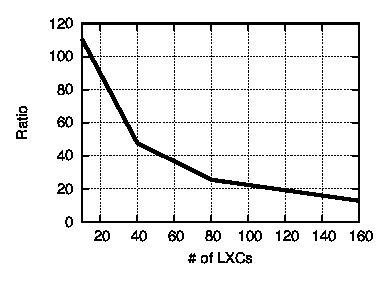
\includegraphics[width=0.8\textwidth]{images/over_3ms_xn.eps} \\ 
      {\textbf{(a) 6 Dedicated CPUs and 24 GB RAM}}\label{subfig-1:over_small} \\ 
      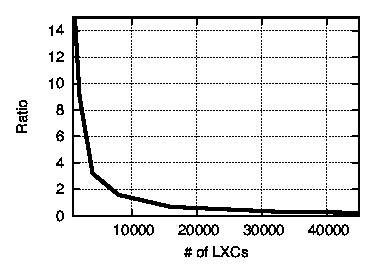
\includegraphics[width=0.8\textwidth]{images/over_3ms_xn_large.eps} \\ 
      {\textbf{(b) 28 Dedicated CPUs and 64 GB RAM}}\label{subfig-2:over_large} 
  \end{tabular} 
    \caption{Overhead Ratio with Timeslice=3ms as a Function of \#LXCs} 
    \label{fig:overheadxn} 
  \end{figure} 

The overhead ratio calculated on a machine with 32 cores (28 dedicated cores) and 45,000 LXCs was {\bf .23} and is shown in Figure \ref{fig:overheadxn}(b). This is to be expected, and reducing that overhead will be explored in the following section.  
\subsection{Optimizing the Synchronization Overhead}
As we found previously, when the number of LXCs in an experiment was extremely large the amount of time spent in the synchronization phase dramatically increased. In fact, more time would be spent in the synchronization phase than time spent with allowing the LXCs time to advance! To reduce this overhead, we redesigned the synchronization phase to allow it to be run in parallel, with the work split up among a finite amount of threads. For the experiment, we compared the amount of time spent in the synchronization phase with our new optimized code verse the amount of time spent in the synchronization phase with the original code. We scaled the number of LXCs in the experiment and looked at the overall speedup. For the experiment, we allocated 8 threads for the synchronization phase, and the results can be found in Figure \ref{fig:sync_optimized}.
\begin{figure} \centering
      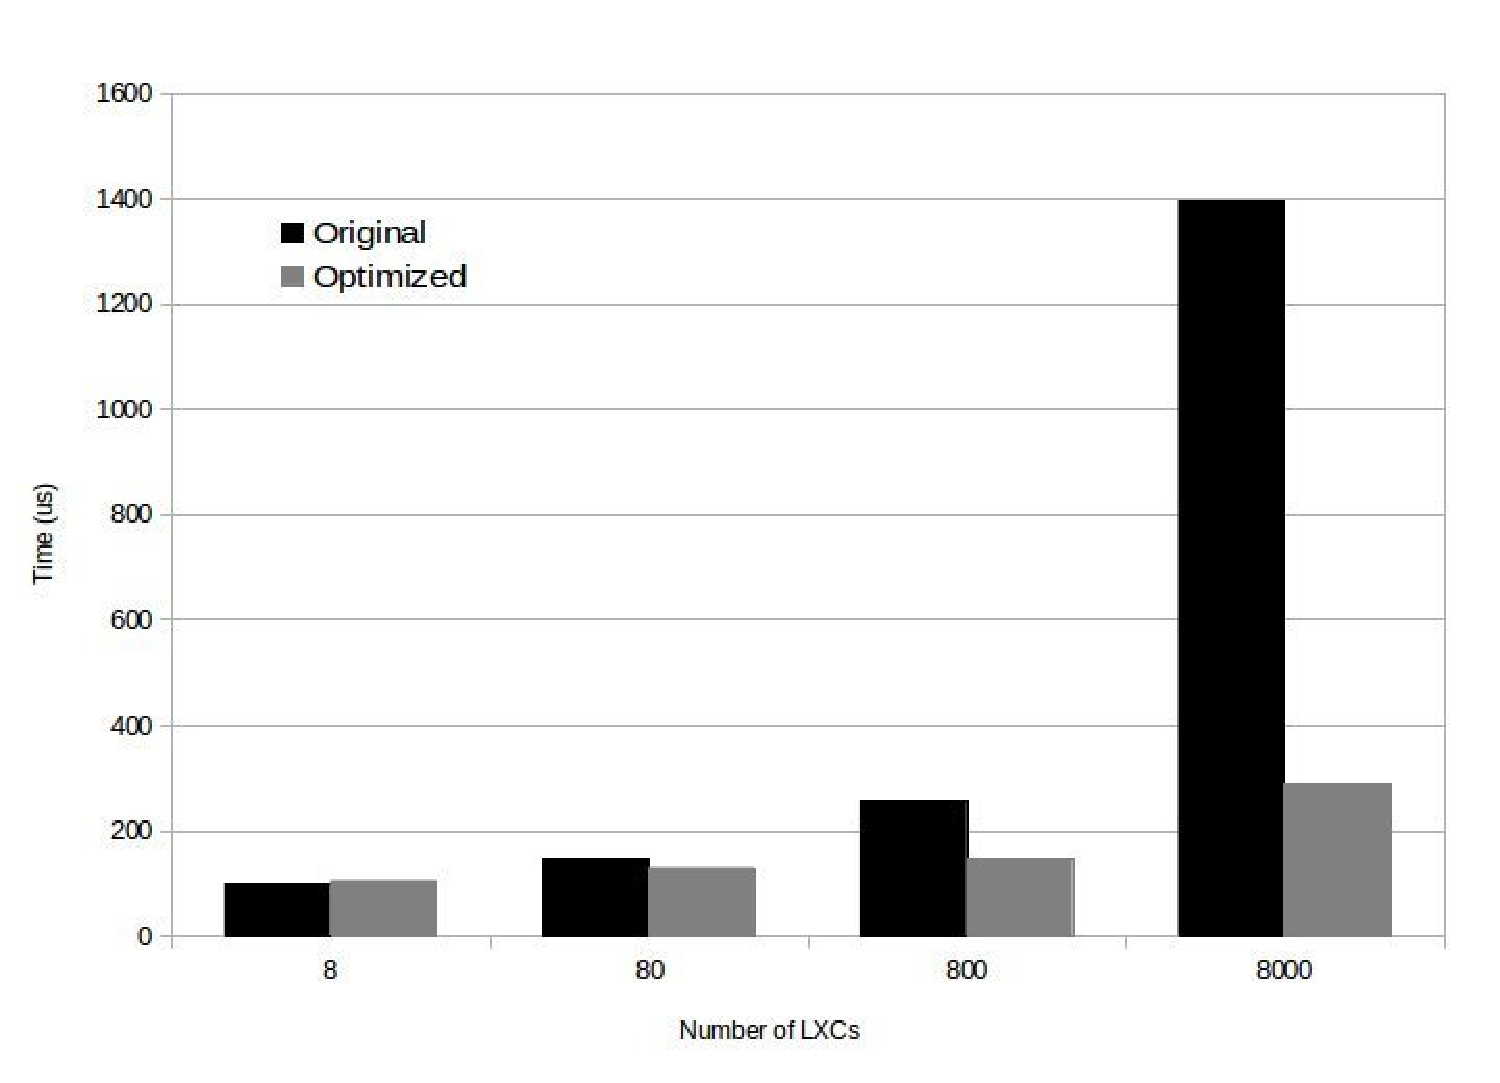
\includegraphics[width=0.8\textwidth]{images/sync_optimized.eps} 
    \caption{Time Spent in the Synchronization Phase} 
    \label{fig:sync_optimized} 
  \end{figure}  
Interestingly, when there are only 8 LXCs in the experiment, the optimized code is actually less efficient than the original code (with a speedup of .94x). This outcome is plausible, as needing to keep the 8 synchronization threads in parallel introduces some additional overhead. When the number of LXCs in the experiment is small, it is actually more efficient for one thread to go through each LXC and do the synchronization computation. However, a high improvement was seen when we ramped up the number of LXCs in the experiment to consist of 8000 LXCs. With 8000 LXCs, we found our optimized code to give us a 4.84x speedup as opposed to the original unoptimized code.
\section{Maintaining Real-Time}
We also wanted to determine how efficient TimeKeeper is at keeping LXCs running in real-time. When we say real-time, we mean that for every instant in time, all LXCs in the experiment will have a virtual time that is greater than or equal to the system time. Obviously, we will only be able to keep an experiment in real-time if all of its TDFs are all less than or equal to 1. For the experiment, we assumed all LXCs have the same TDF. Therefore, the maximum number of LXCs in an experiment we can keep in real-time is: N/TDF, where N is the number of dedicated CPUs on the machine, and we are assuming no overhead. However, our system does have overhead, so our experiment will determine just how close we can get to this upper bound. We ran experiments with 6 dedicated CPUs, a $timeslice$ of 3$ms$, and TDFs of 1/10, 1/50, and 1/100 with increasing numbers of LXCs per experiment, until we found the tipping point (the point where we could no longer keep the experiment as a whole in real- time). We calculated the virtual time of each LXC and compared it to the system time at the end of each $timeslice$ interval. Our results are in Figure \ref{fig:rt}. 

\begin{figure} \centering  
 \begin{tabular}{c} 
      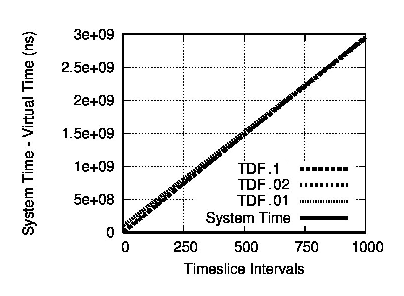
\includegraphics[width=0.8\textwidth]{images/optimal.eps} \\ 
      {\textbf{(a) 6/(TDF+1) \#LXCs}}\label{subfig-1:rtopt} \\ 
      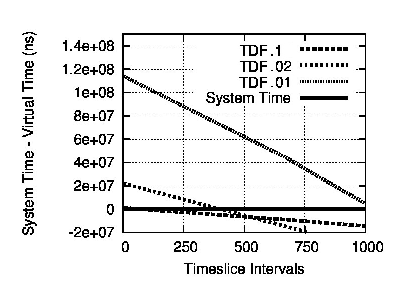
\includegraphics[width=0.8\textwidth]{images/notoptimal.eps} \\ 
      {\textbf{(b) 6/(TDF+1) +1 \#LXCs}}\label{subfig-2:rtnotopt} 
  \end{tabular} 
    \caption{Determining Maximum \#LXCs Where Real-Time is Maintained} 
    \label{fig:rt} 
  \end{figure} 
We found the maximum number of LXCs to be: $6/(TDF+1)$, any more LXCs cause a tipping point and the experiment can no longer be kept in  real-time. Figure \ref{fig:rt}(a) displays the virtual time of the experiment with respect to the system time using this tipping point. As you can see, all experiments virtual time is $increasing$ linearly in respect with the system time. Figure \ref{fig:rt}(b) displays the same thing, but this time, adding just 1 more LXC to each experiment, ie: $6/(TDF+1)+1$. This is obviously the tipping point, as all three experiments virtual time is now $decreasing$ with respect to the system time.
\section{CORE Experiments}
\label {sec:core_experiments}
Here we will discuss experiments conducted with TimeKeeper while it was fully integrated with CORE. 
\subsection{Verifying Network Bandwidth}
The following experiments consisted of basic network analysis with CORE while TimeKeeper is integrated. Within TimeKeeper's notion of a synchronized experiment, some containers may be frozen for large periods of time, allowing other container's time to 'catch up'. Consider the example when one container has a TDF of 10 and another has a TDF of 1. In this scenario, the container with a TDF of 1 will only be allowed to run 1/10 the time of the container with a TDF of 10. Therefore, it is important for the fidelity of the experiment that freezing/unfreezing a container does not interfere with the packet flow of the application. The experiment consisted of a simple 3-node topology, with one switch, one server, and one client. The $iperf$ tool was used to measure the bandwidth between the client and the server. The experiment was repeated numerous times, calculating the average bandwidth, CPU utilization, and experiment length. This process was collected across experiments with varying TDFs, and the results can be found in Figure \ref{fig:core_exp}.
\begin{figure} \centering
 \begin{tabular}{c} 
      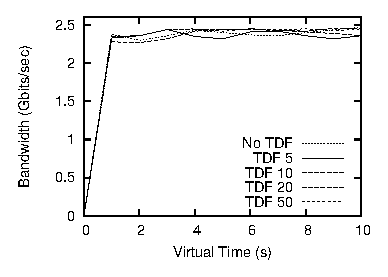
\includegraphics[width=0.8\textwidth]{images/core_iperf.eps} \\ 
      {\textbf{(a) 6/(TDF+1) \#LXCs}}\label{subfig-1:core_iperf} \\ 
      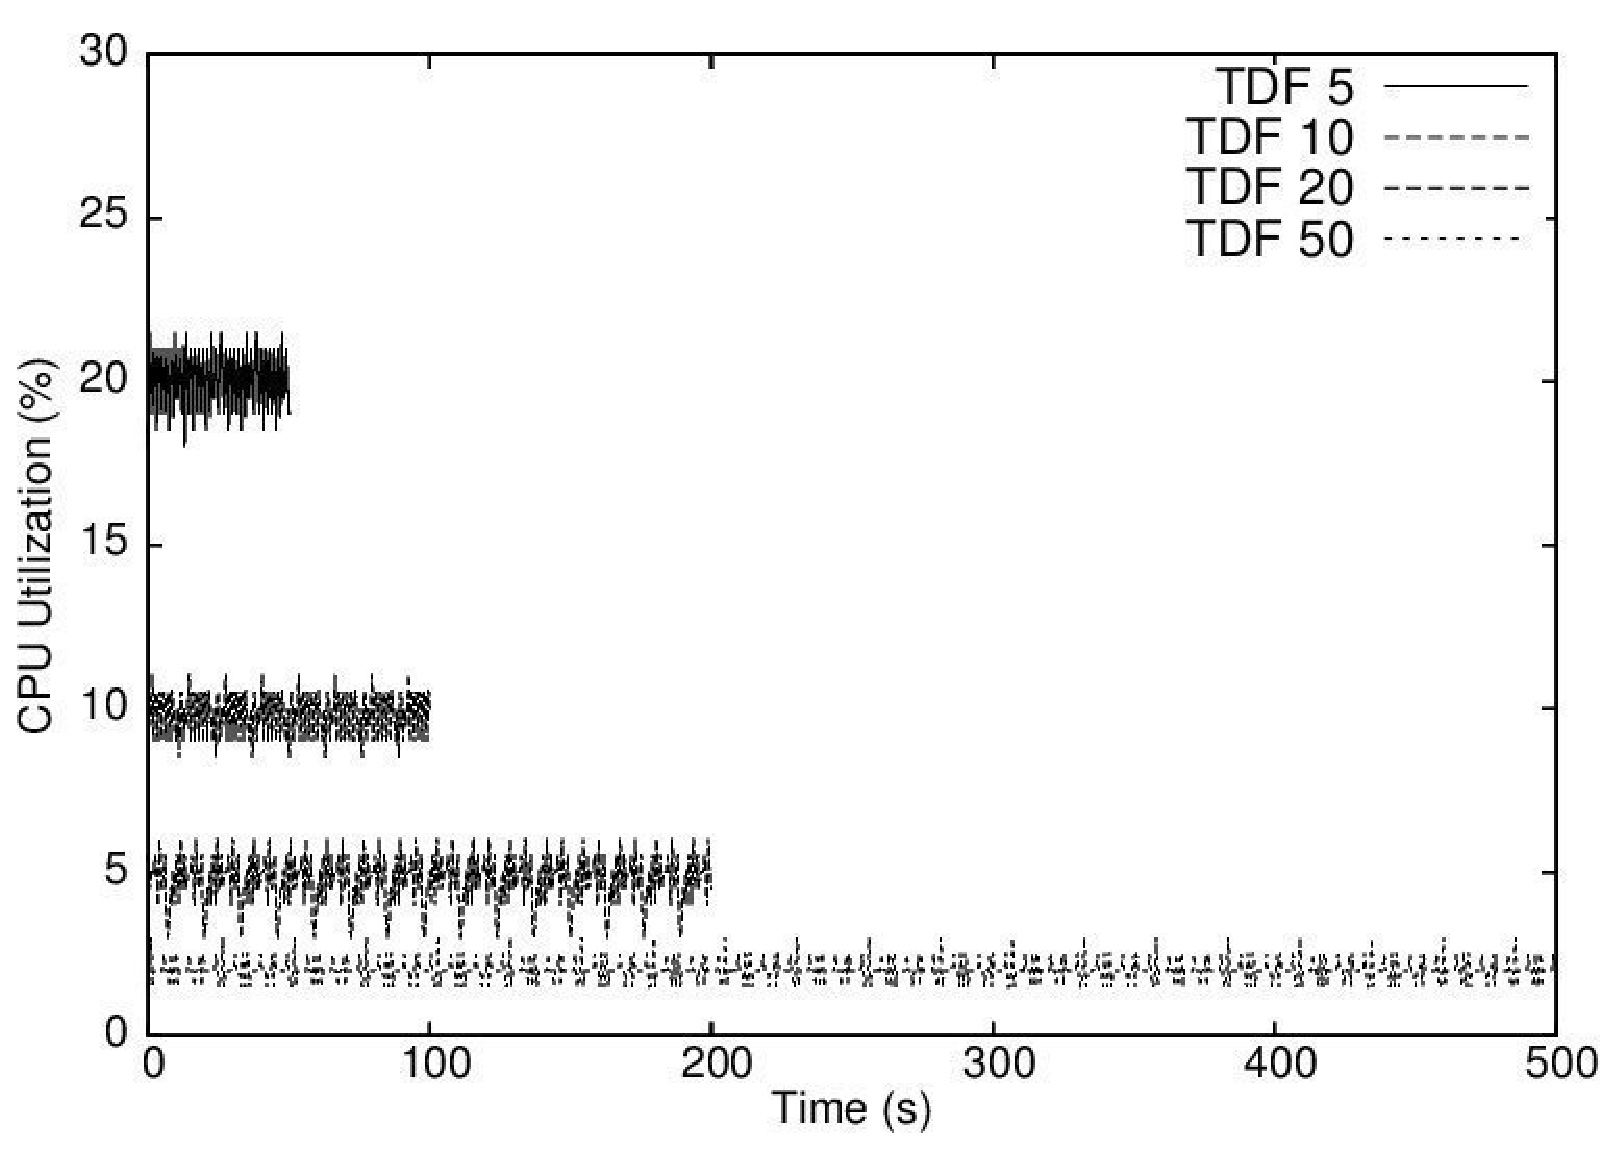
\includegraphics[width=0.8\textwidth]{images/core_cpu.eps} \\ 
      {\textbf{(b) 6/(TDF+1) +1 \#LXCs}}\label{subfig-2:core_cpu} 
  \end{tabular} 
    \caption{Determining Maximum \#LXCs Where Real-Time is Maintained} 
    \label{fig:core_exp} 
  \end{figure} 
Figure \ref{fig:core_exp}(a) displays the resulting bandwidth across time using different TDFs. As you can see, regardless of whether or not the experiment was running in real-time (the case where no TDF is used), or much slower than real-time (where the TDF is 50), the resultant bandwidth is approximately the same. This is very promising, and helps support our claim that a time-dilated experiment will return the same results as an experiment ran without a TDF. Next, Figure \ref{fig:core_exp}(b) explores how different TDFs have an effect on the CPU utilization, as well as the overall time necessary to run an experiment. When the experiment is conducted without a TDF, the $iperf$ process takes approximately 10 seconds to run, and demands 100\% of the CPU in order to send as many packets as possible. This default case is not shown in Figure \ref{fig:core_exp}(b) in order to show in more detail what is going on when the synchronized experiment is assigned a TDF. As the TDF of a synchronized experiment increases, the CPU utilization of the $iperf$ process is decreased with respect to the TDF. However, this comes at the cost of a longer overall experiment runtime. Figure \ref{fig:core_exp}(b) demonstrates that when the TDF of the experiment is 50, the $iperf$ process only spends approximately 2\% of its time on the CPU. However, the same experiment will now takes 500 seconds to run. This tradeoff between system utilization and experiment runtime is beneficial to an extent. A lower system utilization will allow us to run more complex topologies with a network simulator, and this is further explored in Section \ref{sec:ns3_experiments}. \\ 
The previous experiment demonstrated TimeKeeper's ability to maintain a consistent bandwidth with a simple 3-node topology. Here, the experiment was extended to be more complex. This time, an additional 100 containers were added to the experiment, and were configured to randomly send messages to one another. This increases the complexity in two ways. First, the number of containers TimeKeeper needs to synchronize is increased by a factor of 50. Next, additional background traffic is added, as the new containers randomly talk to one another. Once again, the experiment was ran with numerous different TDFs, and the average bandwidth as measured. Similar to the previous experiment, we found the bandwidth to be consistent across all runs. The additional containers did not affect TimeKeeper's ability to maintain a consistent bandwidth; however, it did increase the overall experiment runtime. The overall bandwidth was lower than the overall bandwidth in the previous experiment, but this makes sense as the additional background traffic is running concurrently with the $iperf$ process.
\section{NS-3 Experiments}
\label {sec:ns3_experiments}
Here we will discuss experiments ran with TimeKeeper integrated with ns-3. 
\subsection{Measuring Jitter with a Non-Overloaded Simulator}
In ns-3, $jitter$ is defined as the difference in time between when a event should be processed in the simulator and when the event actually is processed. When running ns-3 with the RealTime Scheduler, reducing the jitter is very important to increase the fidelity of the experiment. When the RealTime Scheduler is running in $Hard Limit$ mode, it will abruptly stop if the jitter gets above a certain point (the default is 100ms). The following experiments were developed to investigate how TimeKeeper may be utilized to reduce the overall jitter within a simulation. First, a simple ns-3 network was created which consisted of a server and a client (both the server and the client were LXCs). Both nodes communicated via the WiFi network model provided by ns-3. We performed an $iperf$ between the client and the server, measuring the jitter for every single event. This procedure was repeated across experiments with many different TDFs. The results are found in Figure \ref{fig:nonoverloaded}.
\begin{figure} \centering  
      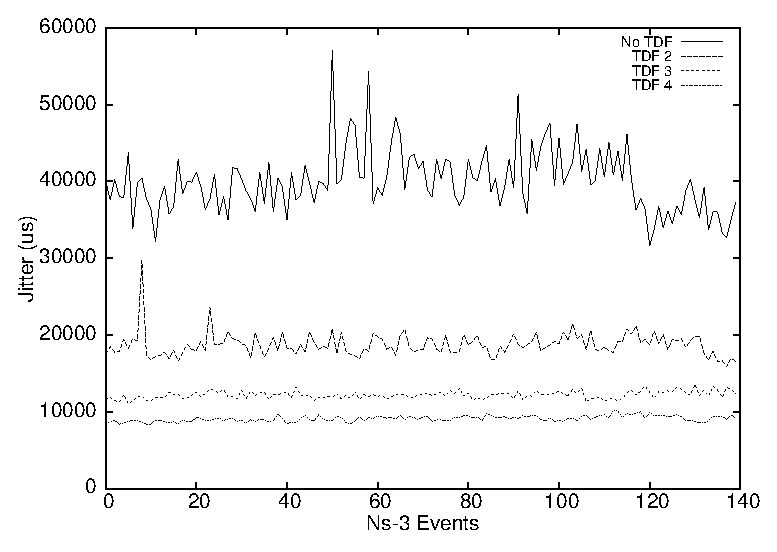
\includegraphics[width=0.8\textwidth]{images/jitter_nonoverloaded.eps} 
    \caption{Jitter Non-Overloaded WiFi Model} 
    \label{fig:nonoverloaded} 
  \end{figure}  
As you can see, the simulator was never overloaded, because for every single experiment the jitter was below the default $HardLimit$ of 100ms. The average jitter for a non time-dilated experiment was about 40ms. When the experiment was repeated with TDFs of 2, 3, and 4, the resulting average jitter was 18.7ms, 12.2ms, and 9.1ms respectively. The reduction in jitter was anticipated, as the TDF specifies how long an experiment should take to run, and the average jitter will be reduced by the factor of the TDF. \\
\subsection{Measuring Jitter with a Overloaded Simulator}
Next, we look at how the jitter is affected when the simulator was overloaded. From the previous CORE experiments (in Section \ref{sec:core_experiments} we learned that with a high TDF the synchronized experiment will progress through virtual time more slowly, thus reducing the stress on the simulator.  Therefore, a simulation which was previously overloaded should be able to complete and give accurate results if given a high enough TDF. To create an overloaded experiment, we constructed a simple ns-3 network using the CSMA network model. Once again, we had a client and a server, and the  client would perform an $iperf$ to measure the bandwidth. This situation originally overloads the simulator, because the CSMA network model attempts to provide higher bandwidth than the WiFi network model, and the additional packet events bog down the simulator. Once again, we recorded the jitter for every event, and repeated this procedure for experiments with different TDFs. The results are found in Figure \ref{fig:overloaded}.
\begin{figure} \centering  
      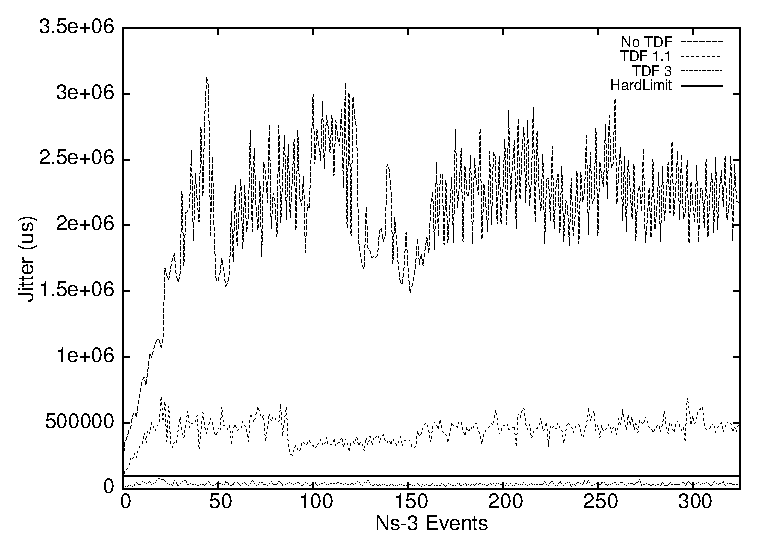
\includegraphics[width=0.8\textwidth]{images/jitter_overloaded.eps} 
    \caption{Jitter Overloaded CSMA Model} 
    \label{fig:overloaded} 
  \end{figure}
  When the simulator was overloaded, the average jitter is hurt dramatically. When the experiment did not have a TDF, the average jitter was 2108ms, or roughly 20x greater than the RealTime Scheduler's default $HardLimit$. An improvement is seen when the experiment is given a TDF of 1.1, which cuts the average jitter down to 441ms. Increasing the experiments TDF to 3 further reduces the average jitter down to 35.4ms. When the TDF is 3, it is considered a successful experiment, as the jitter never exceeds the default $HardLimit$. 
\subsection{Increasing Network Complexity}
While we have demonstrated that increasing the TDF of an experiment will reduce the average jitter in a simple experiment, we wanted to ensure the same held true in a more complicated network as well. This was done by constructing a network topology which consisted of 100 ns-3 nodes. These nodes would communicate with one another over the WiFi network model to provide background traffic, as well as cause extra stress on the ns-3 simulator. In addition, we tied in two LXCs who were connected to the same network model, and performed a $iperf$ test between them. This more complicated topology was able to overload the ns-3 simulator, unlike the previous WiFi network model example. We ran the experiment with various TDFs and calculated the average jitter. The results can be found in Table \ref{table:complexns3}.
\begin{table}\footnotesize\centering 
\begin{tabular}{|c|c|} 
        \hline 
        TDF & Runtime\\ \hline 
        None & 1700ms \\ \hline 
        2 & 738ms \\ \hline 
        3 & 312ms \\ \hline 
        4 &  101ms \\ \hline 
        5 & 30ms \\ \hline 
        10 & 4.25ms \\ \hline 
        \hline 
        \end{tabular} 
        \caption{Average Jitter with Large Ns-3 WiFi Model} 
        \label{table:complexns3} 
\end{table}
Similar to the previous experiment regarding jitter, as the TDF increased the average jitter decreased. When the TDF of the experiment was 5 or 10, the jitter remained under the default $Hard Limit$ of the RealTime Scheduler, and would be able to finish successfully and give accurate results. The size of the experiment did not seem to affect TimeKeeper's ability to reduce the average jitter. We were able to run more complicated experiments that would have previously failed out or given inaccurate results. This is done setting a high experiment TDF to reduce the average jitter; however, it is important to remember that this comes at the cost of higher experiment runtime.
\section{Current Limitations}
\label{sec:limitations}
In this section, we will discuss a comprehensive list of TimeKeeper's limitations. We will describe how these limitations do not prevent TimeKeeper from achieving its design goals. 
\subsection{Adequate Hardware}
TimeKeeper will be limited in its ability to function properly if the system in which it is installed on is relatively old. Here, relatively old is considered to be a system where it only has one or two vCPUs (even with hyperthreading), and less than 4 GB of RAM. This system would not be ideal for TimeKeeper, as the user needs to set specific vCPUs in which TimeKeeper will be allowed complete control. If there are only one or two such vCPUs, TimeKeeper will most likely overload the system, and normal background Linux tasks will not be able to complete. Therefore, it is imperative TimeKeeper is installed on a system with at least four vCPUs. We do not think this is an outrageous demand, as most standard laptops on the market currently start out with four vCPUs. 
\subsection{Manipulating LXCs Correctly}
There are two standard ways in which most people use LXCs. One method creates the LXC and starts a bash terminal. From here, the user can manually interact with this terminal by running various commands and scripts. TimeKeeper directly supports this method, and has no problems. The other method is to start the LXC as a daemon, and use the $lxc$-$attach$ tool to run specific commands from within the LXC. This is more common if you want to create many LXCs, and having so many open terminals would be extremely cumbersome. Here is where a problem arises with TimeKeeper. Recall TimeKeeper interacts with a LXC and all of the LXC's children via a linked list in the $task\_struct$. The process created from $lxc$-$attach$ is not actually a child of the LXC; rather, it is created externally and then pushed into the LXC's namespace. Therefore, TimeKeeper is not able to handle this new process correctly, as it is not technically a child of the LXC, and not found when TimeKeeper traverses the LXC's linked list of children. However, a workaround was developed to quickly and easily run commands from within LXC daemons, and the process is outlined in Figure \ref{fig:lxc_commands}. 
\begin{figure}[t] 
      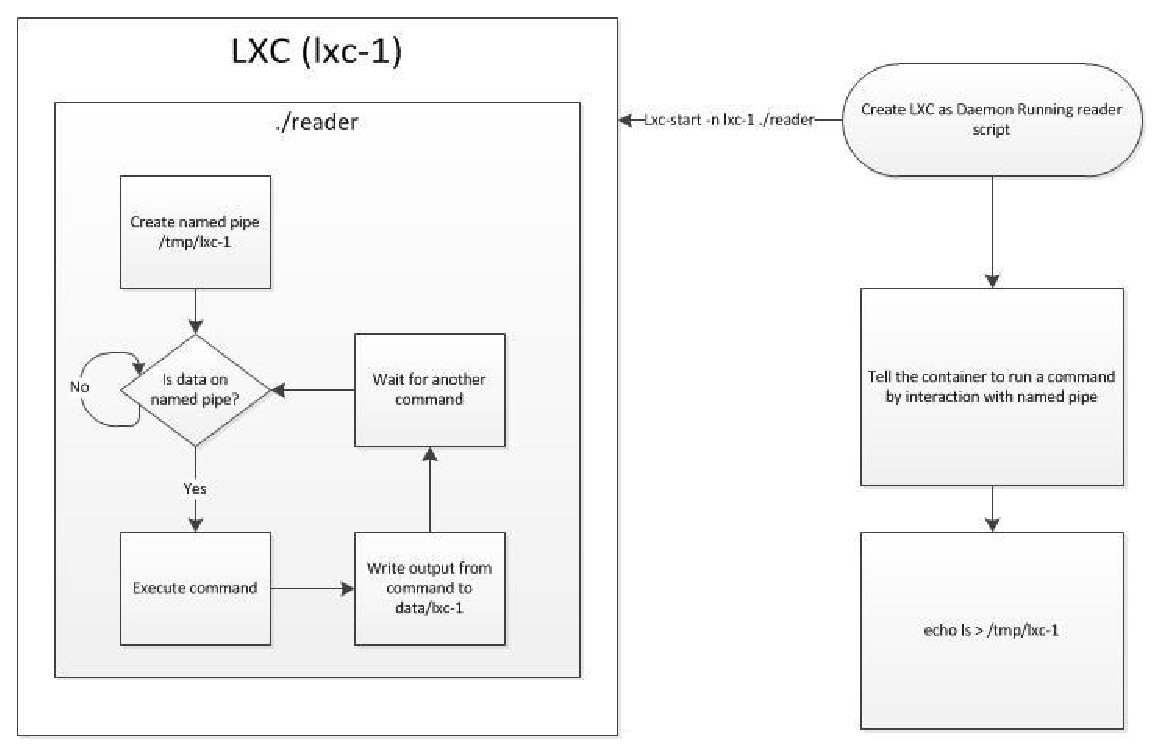
\includegraphics[width=\textwidth]{images/lxc_commands.eps} 
    \caption{Running Commands From Within an LXC Daemon} 
    \label{fig:lxc_commands}
  \end{figure}
For example, lets use $lxc$-$1$ for the name of the LXC. We start the LXC as a daemon with the command $lxc$-$start\ $-$n\ lxc$-$1\ $-$d\ ./reader$. The $reader$ script will get executed when the daemon is started. All the $reader$ script will do is create a named pipe in the /tmp directory based on the name of the LXC, and wait for data to be sent to the named pipe. When data arrives, the $reader$ will try to execute whatever was sent, and store the output of the command in a data directory. So to have the LXC run the $ls$ command to print the files in the current directory, you simply need to run $echo\ ls\ >\ /tmp/lxc$-$1$. To see the output of running the command, simply read data/lxc-1. This method allows us to quickly spawn up many daemons and have them run commands simultaneously with TimeKeeper functioning properly.
\subsection{Kernel Crashes}
It is nearly impossible to claim a complex LKM to be completely bug free, and TimeKeeper is no exception. If the user runs TimeKeeper as it was intended, and uses the API functions in the correct order, TimeKeeper will rarely crash. However, there still exist some edge cases TimeKeeper does not correctly handle if things do not go as planned. In this case, TimeKeeper will most likely crash, and the computer will need to be restarted before TimeKeeper can be run correctly again. 
\subsection{Distributed TimeKeeper}
Currently, TimeKeeper only brings a notion of virtual time to one physical system. It is currently not possible to have two separate machines achieving virtual time synchronization simultaneously. Distributed TimeKeeper would be a great idea for future work. The ability to spread TimeKeeper out over multiple machines, or even a physical testbed, would allow for much larger experiments than previously possible.

%\include{conclusion}


\end{document}
\endinput
